\documentclass[12pt,prb,aps]{revtex4-1}
\usepackage {amsmath}
\usepackage{amssymb}
\pdfoutput = 1 
\usepackage {graphicx}
\newcommand{\bomega}{\mbox{\boldmath$\omega$}}
\allowdisplaybreaks

\begin{document}

\title{Inverse Aspect-Ratio Expanded Tokamak Equilibria}
\author{R.~Fitzpatrick\,\footnote{rfitzp@utexas.edu}}
\affiliation{Institute for Fusion Studies,  Department of Physics,  University of Texas at Austin,  Austin TX 78712, USA}
\begin{abstract}
Following Greene, Johnson \& Weimer  [Phys.\  Fluids  {\bf 14}, 671 (1971)] and Connor, Hastie, et alia [Phys.\ Plasmas {\bf 31}, 577 (1988); Plasma Phys.\ Control.\ Fusion {\bf 34}, 161 (1992); Nucl.\ Fusion {\bf 33}, 1553 (1993)],  the
Grad-Shafranov equation for an axisymmetric tokamak plasma equilibrium  is solved via an expansion in the, supposedly small,  inverse aspect-ratio of the plasma, $\epsilon$. 
The displacements of equilibrium magnetic flux-surfaces due to plasma shaping are assumed to be ${\cal O}(\epsilon)$ smaller than the minor radii
of the surfaces, but no other restriction is placed on the nature of the shaping. The solution of the Grad-Shafranov
equation is matched  to a vacuum solution that extends to infinity, and consists of an expansion in toroidal functions. The external poloidal magnetic
field generated by a finite set of discrete external poloidal magnetic field-coils is calculated, and incorporated  into the toroidal function expansion. 
In this manner, the shape of a large aspect-ratio tokamak plasma is directly related to the currents flowing in the external poloidal field-coils. 
Finally, a pedestal in the plasma pressure, and the associated spike in the bootstrap
current, are incorporated into the model.  
\end{abstract}
\maketitle

\section{Introduction}
In a celebrated paper, published in 1971, Greene, Johnson \& Weimer (GJW) developed a theory of axisymmetric tokamak
equilibria that is based on an expansion of the Grad-Shafranov equation (see Sect.~\ref{gs1}) in the inverse aspect-ratio of the plasma (i.e., the ratio of the minor to the  major radius of the plasma torus).\cite{greene} In addition, GJW demonstrated how to  match the
plasma magnetic field to a curl-free magnetic field, in the vacuum region exterior to the plasma,  by distinguishing between the field generated in the vacuum region by currents flowing within the plasma 
and the field generated by external magnetic field-coils. 

GJW assumed that the horizontal (Shafranov) shift\,\cite{shaf} of the plasma magnetic flux-surfaces is
${\cal O}(\epsilon)$ smaller than the minor radius, where $\epsilon\ll 1$ is the inverse aspect-ratio. Furthermore, GJW assumed that the
ellipticity of the flux-surfaces is ${\cal O}(\epsilon)$ smaller than the horizontal shift. This latter assumption was reasonable for the tokamak plasmas, 
characterized by almost circular boundaries in the poloidal plane, that were prevalent in the 1960s and 1970s. Nowadays, however,  tokamak plasmas
are  highly elongated and strongly shaped in the poloidal plane.\cite{wesson}  Starting in 1985,  in a series of papers, Connor, Hastie, et alia (CHA) generalized the GJW analysis to
allow for flux-surface elongation and triangularity that is of the same order of magnitude as the horizontal shift. \cite{con0,con,gim,fitz93}
However, CHA did not perform the vacuum matching procedure. Moreover, CHA assumed that the plasma is
up-down symmetric. Nowadays, however, tokamak plasmas tend to have a lower magnetic null on the plasma boundary that render them significantly up-down asymmetric.\cite{wesson}  Tokamak plasmas also generally feature a pedestal in the plasma pressure, close to the plasma boundary, with an associated
spike in the parallel current density due to the bootstrap current.\cite{wesson}

The aim of this paper is to generalize the analysis of GJW and CHA so as to allow for strong magnetic flux-surface shaping of a general nature, lack of up-down symmetry,
and the presence of a pedestal in the plasma pressure profile. 
Furthermore, we wish to perform the matching to the vacuum solution, with the eventual aim of directly relating the shape of the plasma to
currents flowing in a set of discrete external poloidal magnetic field-coils. 

Despite the widespread availability of fast numerical solvers for the Grad-Shafranov equation,\cite{helena,chease} analytic model equilibria are still widely used by fusion scientists,\cite{sol,model,model1} particularly in preliminary design studies. Most of these model equilibria are extensions of the 
model equilibria first discovered by Solov'ev in the 1960s.\cite{sol}  Solov'ev-type equilibria have the property that the plasma current profile extends all the way to the plasma
boundary, necessitating a large discontinuous jump in the  current density across the plasma/vacuum interface. Such a jump has a highly
destabilizing influence on ideal external-kink modes,\cite{fred}  which generally means that Solov'ev-type equilibria are unsuitable for free-boundary plasma 
stability 
calculations. On the other hand, the aspect-ratio expanded model equilibria of GJW and CHA allow the plasma current density to go to zero at the
plasma boundary, eliminating the need for a discontinuous jump in the plasma current density across the plasma/vacuum interface. Hence, such equilibria are
quite suitable for free-boundary plasma stability calculations. 

Conventional numerical solvers for the Grad-Shafranov equation, such as HELENA and CHEASE,\cite{helena,chease} only calculate the solution
inside the plasma boundary, and, hence, do not provide the vacuum solution outside the boundary.  Reference \onlinecite{xu}  demonstrates how a
vacuum solution can be added to a Solov'ev solution by means of a Green's function.  Moreover, Ref.~\onlinecite{liu} shows how this vacuum solution
can be related to currents flowing in a finite set of discrete poloidal magnetic field-coils surrounding the plasma. Such a vacuum solution can easily be added to a HELENA or a CHEASE solution using similar techniques. Unfortunately, the numerical implementation of a general Green's function solution is extremely time consuming. One of the main advantages of the GJW and CHA model equilibria is that  most of the hard work entailed in  the calculation of the vacuum
solution can be performed by means of analysis, so that the numerical implementation of the solution can be carried out very rapidly. 

This paper is organized as follows. In Sect.~\ref{splasma}, we discuss the equilibrium solution inside the plasma. In
Sect.~\ref{svac}, we match the plasma solution to a generic vacuum solution outside the plasma. In Sect.~\ref{scoil}, we match the plasma solution to
the vacuum solution generated by a set of discrete external poloidal  magnetic field-coils. Pedestal physics is
discussed in Sect.~\ref{sped}. In Sect.~\ref{sexample}, we describe some example calculations. (Note that, given the great efficiency of the analytic
expansion method described in this paper, all of these calculations can be performed in a fraction of a second on an ordinary laptop computer.) 
Finally, the paper is summarized, and conclusions are drawn, in Sect.~\ref{summary}.

\section{Plasma Solution}\label{splasma}
\subsection{Coordinates}
Consider a tokamak plasma confined on a set of nested, axisymmetric, magnetic flux-surfaces. 
Let $R$, $\phi$, $Z$ be  right-handed cylindrical coordinates whose symmetry axis corresponds to the common
symmetry axis of the flux-surfaces. 
Let us define  right-handed flux-coodinates, $r$, $\theta$, $\phi$, where $r(R,Z)$ is a magnetic flux-surface label with the dimensions
of length, and $\theta(R,Z)$ a poloidal angle. Let\,\cite{con0,con,fitz93}
\begin{equation}\label{e1}
{\cal J} \equiv (\nabla r\times\nabla\theta\cdot\nabla\phi)^{-1} \equiv R\left(\frac{\partial R}{\partial\theta}\,\frac{\partial Z}{\partial r} -\frac{\partial R}{\partial r}\,\frac{\partial Z}{\partial \theta}\right)= \frac{r\,R^{\,2}}{R_0}
\end{equation} 
be the Jacobian of the flux-coordinate system. Here, $(R_0,\, 0)$ are the ($R$, $Z$)  coordinates of the magnetic axis of the nested magnetic flux-surfaces.
The axis  corresponds to $r=0$ in the flux-coordinate system.  
Note that $|\nabla\phi|=R^{\,-1}$. 

\subsection{Equilibrium Magnetic Field and Current}
The divergence-free equilibrium magnetic field is written\,\cite{greene}
\begin{equation}\label{e2}
{\bf B} = B_0\,R_0\left[f(r)\,\nabla\phi\times \nabla r+g(r)\,\nabla\phi\right],
\end{equation}
where $f(r)$ and $g(r)$ are free (dimensionless)  flux-surface functions, and $B_0$ is the toroidal magnetic field-strength at the magnetic axis. 

It is helpful to define the {\em toroidal magnetic flux}\/ (divided by $2\pi$) contained within the magnetic flux-surface whose label is $r$,
\begin{equation}
{\mit\Psi}_t(r)= B_0\int_0^r r'\,g(r')\,dr',
\end{equation}
and the corresponding {\em poloidal magnetic flux}\/ (divided by $2\pi$),
\begin{equation}\label{e4}
{\mit\Psi}_p(r)= B_0\,R_0\int_0^r\,f(r')\,dr'.
\end{equation}
The {\em safety-factor}\/ of the flux-surface (which is the inverse of the rotational transform),\cite{boz}
\begin{equation}\label{e5}
q(r)\equiv \frac{d{\mit\Psi}_t}{d{\mit\Psi}_p} = \frac{r\,g}{R_0\,f},
\end{equation}
is directly related to these two fluxes.

It follows from Eqs.~(\ref{e1}), (\ref{e2}), and (\ref{e5}) that
\begin{equation}
{\bf B} = B_0\,R_0\,f(r)\,\nabla r\times \nabla(q\,\theta -\phi),
\end{equation}
which implies that
\begin{equation}\label{e7y}
\frac{{\bf B}\cdot\nabla \theta}{{\bf B}\cdot\nabla\phi} = \frac{1}{q(r)}.
\end{equation}
Consequently,  if the equilibrium magnetic field-lines within a given  magnetic flux-surface are plotted in the $\theta$-$\phi$
plane then they appear as parallel straight lines whose pitch is determined by the surface's safety-factor (or rotational transform). 

It is also helpful to define the {\em toroidal plasma current}\/ flowing within the flux-surface whose label is $r$,
\begin{equation}\label{e6}
I_t(r)= \frac{1}{2\pi}\int_0^r {\bf j}\cdot\nabla\phi \,{\cal J}\,dr\,d\theta\,d\phi = \frac{2\pi\,B_0}{\mu_0}\,r\,f(r)\,\langle|\nabla r|^2\rangle(r),
\end{equation}
and the corresponding {\em poloidal plasma current},
\begin{equation}\label{e7}
I_p(r)= \frac{1}{2\pi}\int_0^r {\bf j}\cdot\nabla\theta\,{\cal J}\,dr\,d\theta\,d\phi = \frac{2\pi\,B_0\,R_0}{\mu_0}\left[1-g(r)\right].
\end{equation}
Here, ${\bf j}$ is the equilibrium plasma current density.  Moreover, $\langle X\rangle(r) \equiv \oint X(r,\theta)\,d\theta/2\pi$. 
Note that $g(0)=1$, by convention, so as to ensure that $B_0$ is indeed the toroidal magnetic field-strength on the magnetic axis.

\subsection{Equilibrium Magnetic Flux-Surfaces}
The loci of the equilibrium magnetic flux-surfaces are written in the parametric form\,\cite{con0,con,fitz93,greene,gim}
\begin{align}
R(r,\omega) &= R_0-r\,\cos\omega+\sum_{n>0}H_n(r)\,\cos[(n-1)\,\omega]+\sum_{n>1}V_n(r)\,\sin[(n-1)\,\omega]\nonumber\\[0.5ex]&
\phantom{=}+L(r)\,\cos\omega,\label{e10a}\\[0.5ex]
Z(r,\omega)&= r\,\sin\omega + \sum_{n>1}H_n(r)\,\sin[(n-1)\,\omega]- \sum_{n>1}V_n(r)\,\cos[(n-1)\,\omega]\nonumber\\[0.5ex]&\phantom{=}-L(r)\,\sin\omega,\label{e11a}
\end{align}
Here, $H_1(r)$  controls the relative horizontal locations of the flux-surface centroids, respectively, $H_2(r)$ and $V_2(r)$ control the 
up-down symmetric and asymmetric flux-surface ellipticities, respectively, $H_3(r)$ and
$V_3(r)$ control the up-down symmetric and asymmetric flux-surface triangularities, respectively, et cetera, whereas $L(r)$ is a
re-labelling parameter. Moreover, $\omega(R,Z)$ is a  poloidal angle that is distinct from $\theta$.

Let
\begin{equation}
J(r,\omega) = \frac{\partial R}{\partial\omega}\,\frac{\partial Z}{\partial r} -\frac{\partial R}{\partial r}\,\frac{\partial Z}{\partial \omega}
\end{equation}
be the Jacobian of the $r$, $\omega$ coordinate system. We can transform to the $r$, $\theta$ coordinate system 
by writing
\begin{align}\label{e11}
\theta(r,\omega) &= \left.2\pi\int_0^\omega \frac{J(r,\omega')}{R(r,\omega')}\,d\omega'\right/\oint\frac{J(r,\omega)}{R(r,\omega)}\,d\omega,\\[0.5ex]
\frac{r}{R_0}&=\frac{1}{2\pi}\oint\frac{J(r,\omega)}{R(r,\omega)}\,d\omega.\label{e12}
\end{align}
This transformation ensures that 
\begin{equation}
\frac{\partial\theta}{\partial\omega} = \frac{J\,R_0}{r\,R},
\end{equation}
and, hence, that 
\begin{equation}
{\cal J} \equiv R\left(\frac{\partial R}{\partial\theta}\,\frac{\partial Z}{\partial r} -\frac{\partial R}{\partial r}\,\frac{\partial Z}{\partial r}\right)
= R\,J\,\frac{\partial\omega}{\partial\theta} =\frac{r\,R^{\,2}}{R_0},
\end{equation}
in accordance with Eq.~(\ref{e1}). 

\subsection{Grad-Shafranov Equation}\label{gs1}
Equilibrium force balance within the plasma, and the surrounding vacuum,  is governed by the Grad-Shafranov equation,\cite{con0,con,fitz93,greene,gim}
\begin{equation}\label{gs}
\frac{f}{r}\,\frac{\partial}{\partial r}(r\,f\,|\nabla r|^2)+\frac{f}{r}\,\frac{\partial}{\partial\theta}\,(r\,f\,\nabla r\cdot\nabla\theta)
=- g\,\frac{dg}{dr} - \frac{\mu_0}{B_0^{\,2}}\left(\frac{R}{R_0}\right)^2\frac{dp}{dr},
\end{equation}
where $p(r)$ is the equilibrium plasma pressure. Note that we can easily extend the Grad-Shafranov equation to include the centrifugal
effect of plasma flows on the  equilibrium.\cite{flow,flow1} We choose not to do this in the present calculation because such effects are
generally negligible in a  reactor-sized tokamak. 

\subsection{Normalization}
Let $r=a$ correspond to the plasma/vacuum boundary, and let 
\begin{equation}
\epsilon=\frac{a}{R_0}
\end{equation}
 be the {\em inverse-aspect ratio}\/ of the plasma.  It is assumed that $\epsilon\ll 1$. 
Furthermore, let $R=R_0\,\hat{R}$, $Z=R_0\,\hat{Z}$, $r=a\,\hat{r}$, $\nabla = a^{-1}\,\hat{\nabla}$,
 $H_n=\epsilon\,a\,\hat{H}_n$, $V_n=\epsilon\,a\,\hat{V}_n$, and $L=\epsilon^{\,2}\,a\,\hat{L}$. The parametric equations of the flux-surfaces, (\ref{e10a}) and (\ref{e11a}),  become\,\cite{fitz93,gim}
\begin{align}
\hat{R}(\hat{r},\omega) &= 1 -\epsilon\,\hat{r}\,\cos\omega + \epsilon^{\,2}\,\sum_{n>0}\hat{H}_n(\hat{r})\,\cos[(n-1)\,\omega] + \epsilon^{\,2}\,\sum_{n>1}\hat{V}_n(\hat{r})\,\sin[(n-1)\,\omega] \nonumber\\[0.5ex]
&\phantom{=}+\epsilon^{\,3}\,\hat{L}(\hat{r})\,\cos\omega,\label{e19x}\\[0.5ex]
\hat{Z}(\hat{r},\omega)&= \epsilon\,\hat{r}\,\sin\omega +\epsilon^{\,2}\,\sum_{n>1}\hat{H}_n(\hat{r})\,\sin[(n-1)\,\omega]
-\epsilon^{\,2}\,\sum_{n>1}\hat{V}_n(\hat{r})\,\cos[(n-1)\,\omega]\nonumber\\[0.5ex]&\phantom{=}-\epsilon^{\,3}\,\hat{L}(\hat{r})\,\sin\omega.\label{e20x}
\end{align}
It is assumed that, other than $\epsilon$,  all quantities appearing in the previous two expressions are ${\cal O}(1)$. 

\subsection{Metric Elements}
We can determine the metric elements of the flux-coordinate system by combining the previous two equations with Eqs.~(\ref{e11}) and (\ref{e12}). Evaluating the elements up to ${\cal O}(\epsilon)$, but retaining ${\cal O}(\epsilon^{\,2})$ contributions to terms that are independent of
$\omega$, we obtain,\cite{fitz93,gim}
\begin{align}\label{epdef}
\hat{L}(\hat{r})&= \frac{\hat{r}^{\,3}}{8} -\frac{\hat{r}\,\hat{H}_1}{2}-\frac{1}{2}\sum_{n>1}(n-1)\,\frac{\hat{H}_n^{\,2}}{\hat{r}}
-\frac{1}{2}\sum_{n>1}(n-1)\,\frac{\hat{V}_n^{\,2}}{\hat{r}},\\[0.5ex]
\theta &= \omega+\epsilon\,\hat{r}\,\sin\omega - \epsilon\sum_{n>0}\frac{1}{n}\left[\hat{H}_n'-(n-1)\,\frac{\hat{H}_n}{\hat{r}}\right]\sin(n\,\omega)
\nonumber\\[0.5ex]&\phantom{=}+ \epsilon\sum_{n>1}\frac{1}{n}\left[\hat{V}_n'-(n-1)\,\frac{\hat{V}_n}{\hat{r}}\right]\cos(n\,\omega),\label{e22y}\\[0.5ex]
|\hat{\nabla} \hat{r}|^2 &= 1 +2\,\epsilon\sum_{n>0}\hat{H}_n'\,\cos(n\,\theta) +2\,\epsilon\sum_{n>1}\hat{V}_n'\,\sin(n\,\theta) \nonumber\\[0.5ex]
&\phantom{=}+\epsilon^{\,2}\left(\frac{3\,\hat{r}^2}{4}-\hat{H}_1+
\frac{1}{2}\sum_{n>0}\left[\hat{H}_n'^{\,2}+(n^2-1)\,\frac{\hat{H}_n^{\,2}}{\hat{r}^{\,2}}\right]\right.\nonumber\\[0.5ex]&\phantom{=}\left.+
\frac{1}{2}\sum_{n>1}\left[\hat{V}_n'^{\,2}+(n^2-1)\,\frac{\hat{V}_n^{\,2}}{\hat{r}^{\,2}}\right]
\right),\label{e19}\\[0.5ex]
\hat{\nabla}\hat{r}\cdot\hat{\nabla}\theta&=\epsilon\,\sin\theta
-\epsilon\sum_{n>0}\frac{1}{n}\left[\hat{H}_n''+\frac{\hat{H}_n'}{\hat{r}}+(n^2-1)\,\frac{\hat{H}_n}{\hat{r}^{\,2}}\right]\sin(n\,\theta)\nonumber\\[0.5ex]&
\phantom{=}+\epsilon\sum_{n>1}\frac{1}{n}\left[\hat{V}_n''+\frac{\hat{V}_n'}{\hat{r}}+(n^2-1)\,\frac{\hat{V}_n}{\hat{r}^{\,2}}\right]\cos(n\,\theta)
\nonumber\\[0.5ex]&\phantom{=}
+\epsilon^{\,2}\,\frac{1}{2}\left[\sum_{n>1}(n-1)\left(\frac{\hat{V}_n'\,\hat{H}_n}{\hat{r}^{\,2}}-
\frac{\hat{H}_n'\,\hat{V}_n}{\hat{r}^{\,2}}\right)\right.\nonumber\\[0.5ex]&\phantom{=}\left.
+\sum_{n>1}\left(\frac{n-1}{n}\right)\left(\frac{\hat{V}_n''\,\hat{H}_n}{\hat{r}}-\frac{\hat{H}_n''\,\hat{V}_n}{\hat{r}}\right)
+\sum_{n>1}\frac{1}{n}\left(\hat{V}_n''\,\hat{H}_n'-\hat{H}_n''\,\hat{V}_n'\right)
\right],
\\[0.5ex]
\hat{R}^{\,2}&= 1-2\,\epsilon\,\hat{r}\,\cos\theta -\epsilon^{\,2}\left(\frac{\hat{r}^{\,2}}{2}-\hat{r}\,\hat{H}_1'-2\,\hat{H}_1\right).\label{e25a}
\end{align}
Here, $'\equiv d/d\hat{r}$, and $n$ is a non-negative integer. 

\iffalse
According to Eqs.~(\ref{e7y}) and (\ref{e22y}), the equation of a magnetic field-line in the $\hat{r}$, $\omega$ coordinate system
is
\begin{align}
\frac{d\omega}{d\phi}& = \frac{1}{q(\hat{r})}\left\{1-\epsilon\,\hat{r}\,\cos\omega + \epsilon
\sum_{n>0}\left[\hat{H}_n'-(n-1)\,\frac{\hat{H}_n}{\hat{r}}\right]\cos(n\,\omega) \right.\nonumber\\[0.5ex]&\phantom{+}\left.+\epsilon
\sum_{n>0}\left[\hat{V}_n'-(n-1)\,\frac{\hat{V}_n}{\hat{r}}\right]\sin(n\,\omega)+{\cal O}(\epsilon^{\,2})\right\}.
\end{align}
\fi

\subsection{Expansion of Grad-Shafranov Equation}\label{exp}
Let us write
\begin{align}\label{e26v}
\hat{r}\,f(\hat{r}) &= \epsilon\,f_1(\hat{r}) +\epsilon^{\,3}\,\hat{f}_3(\hat{r})+\cdots,\\[0.5ex]
g(\hat{r}) &= 1+ \epsilon^{\,2}\,g_2(\hat{r}) + \epsilon^{\,4}\,g_4(\hat{r})+\cdots,\label{e27v}\\[0.5ex]
\frac{\mu_0\,p(\hat{r})}{B_0^{\,2}} &= \epsilon^{\,2}\,p_2(\hat{r}) + \epsilon^{\,4}\,p_4(\hat{r})+\cdots,
\end{align}
where $f_1$, $f_3$, $g_2$, $g_4$, $p_2$ and $p_4$ are all ${\cal O}(1)$. It follows from Eq.~(\ref{e5}) that, 
to lowest order in our expansion, the safety-factor profile is given by
\begin{equation}
q_0(\hat{r}) = \frac{\hat{r}^{\,2}}{f_1(\hat{r})},
\end{equation}
whereas, to second order,  the profile takes the modified form 
\begin{equation}\label{e26a}
q_2(\hat{r}) = \frac{\hat{r}^{\,2}}{f_1(\hat{r})}
\left[1+\epsilon^{\,2}\,g_2(\hat{r}) - \epsilon^{\,2}\,\frac{f_3(\hat{r})}{f_1(\hat{r})}\right].
\end{equation}

 Expanding the Grad-Shafranov equation, (\ref{gs}), order by order in the
small parameter $\epsilon$, making use of Eqs.~(\ref{e19})--(\ref{e25a}), we obtain\,\cite{con0,con,greene,gim}
\begin{align}
g_2'&=- p_2' - \frac{f_1\,f_1'}{\hat{r}^{\,2}},\label{e26}\\[0.5ex]
\hat{H}_1''&= -\left(\frac{2\,f_1'}{f_1}-\frac{1}{\hat{r}}\right)\hat{H}_1' 
-1+\frac{2\,\hat{r}^{\,3}\,p_2'}{f_1^{\,2}},\label{e27}\\[0.5ex]
\hat{H}_n''&= -\left(\frac{2\,f_1'}{f_1}-\frac{1}{\hat{r}}\right)\hat{H}_n'+(n^2-1)\,\frac{\hat{H}_n}{\hat{r}^{\,2}}~~~~~\mbox{for $n>1$},\label{e33x}\\[0.5ex]
\hat{V}_n''&= -\left(\frac{2\,f_1'}{f_1}-\frac{1}{\hat{r}}\right)\hat{V}_n'+(n^2-1)\,\frac{\hat{V}_n}{\hat{r}^{\,2}}~~~~~~\,\mbox{for $n>1$},\label{e28}\\[0.5ex]
\hat{r}^2\,p_4'+\hat{r}^2\,g_4'+(f_1\,f_3)'&=F_3(\hat{r}),\label{e30}
\end{align}
where
\begin{align}
F_3(\hat{r}) &= -\frac{f_1^{\,2}}{\hat{r}}\left(
\frac{3\,\hat{r}^{\,2}}{2}-2\,\hat{r}\,\hat{H}_1'\right.\nonumber\\[0.5ex]
&\phantom{===}
+\sum_{n>0}\left[\hat{H}_n'^{\,2}+2\,(n^2-1)\,\frac{\hat{H}_n'\,\hat{H}_n}{\hat{r}}-(n^2-1)\,\frac{\hat{H}_n^{\,2}}{\hat{r}^{\,2}}\right]\nonumber\\[0.5ex]
&\phantom{===}\left.+\sum_{n>1}\left[\hat{V}_n'^{\,2}+2\,(n^2-1)\,\frac{\hat{V}_n'\,\hat{V}_n}{\hat{r}}-(n^2-1)\,\frac{\hat{V}_n^{\,2}}{\hat{r}^{\,2}}\right]\right)\nonumber\\[0.5ex]
&\phantom{=}
+f_1\,f_1'\left(g_2-\frac{3\,\hat{r}^{\,2}}{4} +\hat{H}_1 +\frac{1}{2}\sum_{n>0}\left[3\,\hat{H}_n'^{\,2}- (n^2-1)\,\frac{\hat{H}_n^{\,2}}{\hat{r}^{\,2}}\right]
\right.\nonumber\\[0.5ex]
&\phantom{===}\left.+\frac{1}{2}\sum_{n>1}\left[3\,\hat{V}_n'^{\,2}- (n^2-1)\,\frac{\hat{V}_n^{\,2}}{\hat{r}^{\,2}}\right]\right)\nonumber\\[0.5ex]
&\phantom{=}
+\hat{r}^{\,2}\,p_2'\left(g_2+\frac{\hat{r}^{\,2}}{2}-3\,\hat{r}\,\hat{H}_1'-2\,\hat{H}_1\right).\label{e31}
\end{align}
Note that the relative horizontal shift of magnetic flux-surfaces, $\hat{H}_1$, otherwise known as the {\em Shafranov shift},\cite{shaf} is driven by toroidicity [the second term on
the right-hand side of Eq.~(\ref{e27})], and plasma pressure gradients (the third term). All of the other shaping terms (i.e., the $\hat{H}_n$ for $n>1$, and
the $\hat{V}_n$ for $n>1$) are driven by currents flowing in external magnetic field-coils. 

In the present study, it is convenient to set $g_4=p_4=0$. However, other choices are possible. 

\subsection{Plasma Interior}
Let us regard $f_1(\hat{r})$ and $p_2(\hat{r})$ as the two free flux-surface functions that
determine the equilibrium. In the plasma interior, which corresponds to $0\leq\hat{r}\leq 1$, Eq.~(\ref{e26}) yields
\begin{align}
g_2(\hat{r}) &=p_2(0)-p_2(\hat{r}) - \int_0^{\hat{r}}\frac{f_1(\hat{r}')\,f_1'(\hat{r}')}{\hat{r}'^{\,2}}\,d\hat{r}'.\label{e35x}
\end{align}
At small $\hat{r}$, assuming that $f_1(\hat{r})=f_{1\,c}\,\hat{r}^{\,2}$ and $p_2(\hat{r})=p_{2\,c}+(1/2)\,p_{2\,c}''\,\hat{r}^{\,2}$, where $f_{1\,c}$, $p_{2\,c}$,  $p_{2\,c}''$
are constants that can be determined from the given $f_1(\hat{r})$ and $p_2(\hat{r})$ functions, 
we deduce that $g_2(\hat{r}) = -(f_{1\,c}^{\,2}+p_{2\,c}''/2)\,\hat{r}^{\,2}$. Note that we have set $g_2=0$ at $\hat{r}=0$ in order to ensure that $B_0$ is
indeed the toroidal magnetic field-strength on the magnetic axis.
Equation~(\ref{e27}) must be solved subject to the boundary conditions that
\begin{equation}\label{e38vv}
\hat{H}_1(\hat{r}) = \frac{1}{8}\left(\frac{2\,p_{2\,c}''}{f_{1\,c}^{\,2}}-1\right)\hat{r}^{\,2}
\end{equation}
at small $\hat{r}$.  Likewise, Eqs.~(\ref{e33x}) and (\ref{e28}) must be solved subject to the small-$\hat{r}$ boundary conditions that 
\begin{align}
\hat{H}_n(\hat{r}) &= \hat{H}_{n\,c}\,\hat{r}^{\,n-1}~~~~~\mbox{for $n>1$},\\[0.5ex]
\hat{V}_n(\hat{r}) &= \hat{V}_{n\,c}\,\hat{r}^{\,n-1}~~~~~\,\,\mbox{for $n>1$}.\label{e40vv}
\end{align}
Here, $\hat{H}_{n\,c}$ and $\hat{V}_{n\,c}$ are  arbitrary constants. It turns out that the only solution of Eq.~(\ref{e28}) for $n=1$ that does not
blow up at $\hat{r}=0$ is the trivial solution
$\hat{V}_1(\hat{r}) = \hat{V}_{1\,c}$.
However, we wish to set $\hat{H}_1=\hat{V}_1=0$ at $\hat{r}=0$, in
order to ensure that $\hat{r}=0$ is indeed the magnetic axis. Hence, we are forced to conclude that
$\hat{V}_1(\hat{r}) = 0$, which accounts for the absence of this term in our analysis. 
Once we have determined $g_2(\hat{r})$,  as well as the $\hat{H}_n(\hat{r})$ and the $\hat{V}_n(\hat{r})$ functions, we can integrate Eq.~(\ref{e30}) to give 
\begin{align}
f_3(\hat{r})&= \frac{1}{f_1(\hat{r})}\int _0^{\hat{r}}F_3(\hat{r}')\,d\hat{r}'.\label{e36x}
\end{align}
Note that $f_3(\hat{r})=-f_{1\,c}\,(\hat{H}_{2\,c}^{\,2}+\hat{V}_{2\,c}^{\,2})\,\hat{r}^{\,2}$ at small $\hat{r}$. Furthermore, we
have conveniently set $\hat{f}_3=0$ at $\hat{r}=0$, which ensures that $q(0)= [1+\epsilon^{\,2}\,(\hat{H}_{2\,c}^{\,2}+\hat{V}_{2\,c}^{\,2})]/f_{1\,c}$. 

\subsection{Near-Vacuum Region}
We expect 
\begin{equation}\label{e39c}
p_2(\hat{r})=0
\end{equation}
 in the vacuum region immediately surrounding the plasma, which corresponds to $1<\hat{r}\ll \epsilon^{-1}$. We
also expect this so-called {\em near-vacuum region}\/ to be current-free, which implies that $I_t(\hat{r})=I_t(1)$ and $I_p(\hat{r})=I_p(1)$ for 
$\hat{r}>1$. It follows from Eq.~(\ref{e7}) that 
\begin{equation}\label{eg2a}
g_2(\hat{r})= g_{2\,a}
\end{equation}
 in the near-vacuum region, where $g_{2\,a}=g_2(1)$ is a constant determined from Eq.~(\ref{e35x}). 
Likewise, Eq.~(\ref{e6}) requires that
\begin{equation}
\frac{d}{d\hat{r}}\!\left(\hat{r}\,f\,\langle |\hat{\nabla} r|^2\rangle\right)=0
\end{equation}
in the region $\hat{r}>1$. Making use of the orderings introduced in Sect.~\ref{exp}, we deduce that
\begin{equation}\label{e34}
f_1(\hat{r})= f_{1\,a}
\end{equation}
to lowest order, where $f_{1\,a}=f_1(1)$ is a constant that can be determined from the given $f_1(\hat{r})$ profile, and 
\begin{equation}\label{e33}
f_3'(\hat{r}) = -f_{1\,a}\frac{d\langle|\hat\nabla\hat{r}|^2\rangle_2}{d\hat{r}}
\end{equation}
to next order. Here, 
\begin{align}
\langle |\hat\nabla\hat{r}|^2\rangle_2&=
\frac{3\,\hat{r}^2}{4}-\hat{H}_1+
\frac{1}{2}\sum_{n>0}\left[\hat{H}_n'^{\,2}+(n^2-1)\,\frac{\hat{H}_n^{\,2}}{\hat{r}^{\,2}}\right]+
\frac{1}{2}\sum_{n>1}\left[\hat{V}_n'^{\,2}+(n^2-1)\,\frac{\hat{V}_n^{\,2}}{\hat{r}^{\,2}}\right]\label{e35t}
\end{align}
is the component of $\langle |\hat\nabla\hat{r}|^2\rangle$ that is second order in $\epsilon$. [See Eq.~(\ref{e19}).] 

The toroidal and poloidal current profiles in the plasma can be written $I_{t}(r)= \epsilon^{\,2}\,(B_0\,R_0/\mu_0)\,\hat{I}_t(\hat{r})$ and $I_{p}(r)=  \epsilon^{\,2}\,(B_0\,R_0/\mu_0)\,\hat{I}_p(\hat{r})$,  respectively.  It follows from Eqs.~(\ref{e6}) and (\ref{e7}) that the total
normalized toroidal and poloidal plasma currents flowing in the plasma are
\begin{align}
\hat{I}_{t\,a} &= 2\pi\left[f_1\left(1+\epsilon^{\,2}\,\langle |\hat\nabla\hat{r}|^2\rangle_2\right)+\epsilon^{\,2}\,f_3\right]_{\hat{r}=1},\\[0.5ex]
\hat{I}_{p\,a}&=2\pi\,g_{2\,a},
\end{align}
respsectively. 

In this paper, we shall assume that the equilibrium plasma current density is continuous across the plasma/vacuum interface, as is generally the case in a realistic tokamak plasma (assuming that the plasma current profile has been given sufficient time to diffuse across the plasma). Given that  
the current density is zero in the vacuum region, it follows that the current density must be zero just inside the plasma boundary. In other words,
we require that 
$\hat{I}_t'(1) = \hat{I}_p'(1)= 0$.
Thus,  making use of Eqs.~(\ref{e6}) and (\ref{e7}), we deduce that $g_2'(1)=0$, 
\begin{equation}\label{f2p}
f_1'(1) = 0,
\end{equation}
and also that Eq.~(\ref{e33}) must be satisfied at $\hat{r}=1$. Finally, Eq.~(\ref{e26}) yields
\begin{equation}
p_2'(1) = 0.\label{p2p}
\end{equation}

Note that Eq.~(\ref{e26}) is automatically satisfied in the near-vacuum region. Equations~(\ref{e27})--(\ref{e28}), combined with Eq.~(\ref{e39c}) and (\ref{e34}), 
yield
\begin{align}\label{e36y}
\hat{H}_1''&= \frac{\hat{H}_1' }{\hat{r}}
-1,\\[0.5ex]
\hat{H}_n''&= \frac{\hat{H}_n'}{\hat{r}}+(n^2-1)\,\frac{\hat{H}_n}{\hat{r}^{\,2}}~~~~~\mbox{for $n>1$},\label{e37}\\[0.5ex]
\hat{V}_n''&= \frac{\hat{V}_n'}{\hat{r}}+(n^2-1)\,\frac{\hat{V}_n}{\hat{r}^{\,2}}~~~~~~\,\mbox{for $n>1$},\label{e38v}
\end{align}
which can be solved to give\,\cite{greene}
\begin{align}
\hat{H}_1(\hat{r}) &= \hat{H}_{1\,a} - \frac{\hat{r}^{\,2}}{2}\,\ln\hat{r} +\frac{1}{4}\left(2\,\hat{H}_{1\,a}'+1\right)(\hat{r}^{\,2}-1) ,\label{e37c}\\[0.5ex]
\hat{H}_n(\hat{r}) &= \hat{H}_{n\,a-}\,\hat{r}^{\,n+1} - \hat{H}_{n\,a+}\,\hat{r}^{\,1-n}~~~\mbox{for $n>1$},\\[0.5ex]
\hat{V}_n(\hat{r}) &= \hat{V}_{n\,a-}\,\hat{r}^{\,n+1} - \hat{V}_{n\,a+}\,\hat{r}^{\,1-n}~~~~~\mbox{for $n>1$},\label{e39cx}
\end{align}
in the near-vacuum region. Here, 
\begin{align}
\hat{H}_{n\,a-}&= \frac{\hat{H}_{n\,a}'+(n-1)\,\hat{H}_{n\,a}}{2\,n},\\[0.5ex]
\hat{H}_{n\,a+} &= \frac{\hat{H}_{n\,a}'-(n+1)\,\hat{H}_{n\,a}}{2\,n},\\[0.5ex]
\hat{V}_{n\,a-}&= \frac{\hat{V}_{n\,a}'+(n-1)\,\hat{V}_{n\,a}}{2\,n},\\[0.5ex]
\hat{V}_{n\,a+} &= \frac{\hat{V}_{n\,a}'-(n+1)\,\hat{V}_{n\,a}}{2\,n}.
\end{align}
Moreover, $\hat{H}_{n\,a}=\hat{H}_n(1)$, $\hat{H}_{n\,a}'=\hat{H}_n'(1)$, $\hat{V}_{n\,a}=\hat{V}_n(1)$,
and $\hat{V}_{n\,a}'=\hat{V}_n(1)$  are constants determined from the solutions of Eqs.~(\ref{e27})--(\ref{e28}) in the plasma interior,
subject to the boundary conditions (\ref{e38vv})--(\ref{e40vv}).  It follows from Eqs.~(\ref{e30}), (\ref{e31}),  (\ref{e39c}), and (\ref{e34}) that
\begin{align}\label{e58g}
f_3'(\hat{r})& = -\frac{f_{1\,a}}{\hat{r}}\left(\frac{3\,\hat{r}^{\,2}}{2}-2\,\hat{r}\,\hat{H}_1' +\sum_{n>0}\left[\hat{H}_n'^{\,2}+2\,(n^2-1)\,\frac{\hat{H}_n'\,\hat{H}_n}{\hat{r}}-(n^2-1)\,\frac{\hat{H}_n^{\,2}}{\hat{r}^{\,2}}\right]\right.\nonumber\\[0.5ex]
&\phantom{=}\left.+\sum_{n>1}\left[\hat{V}_n'^{\,2}+2\,(n^2-1)\,\frac{\hat{V}_n'\,\hat{V}_n}{\hat{r}}-(n^2-1)\,\frac{\hat{V}_n^{\,2}}{\hat{r}^{\,2}}\right]
\right).
\end{align}
However, Eqs.~(\ref{e33})--(\ref{e35t}) and (\ref{e36y})--(\ref{e38v}) can be combined to give exactly the same relation, which confirms that zero toroidal current flows in the near-vacuum
region, and also that the toroidal current density is zero at the plasma boundary.  Equations~(\ref{e37c})--(\ref{e39cx}) and (\ref{e58g}) can be integrated to give
\begin{align}\label{e44}
f_3(\hat{r}) &= f_{3\,a} -\frac{f_{1\,a}}{2}\left[\left(1-2\,\hat{H}_{1\,a}'\right)
\hat{r}^{\,2}\,\ln\hat{r}+\hat{r}^{\,2}\,\ln^2\hat{r}+(1-\hat{H}_{1\,a}'+ \hat{H}_{1\,a}'^{\,2})\,(\hat{r}^{\,2}-1)\right.\nonumber\\[0.5ex]
&\phantom{=} +\sum_{n>1}2\,n\,(n+1)\,\hat{H}_{n\,a-}^{\,2}\,(\hat{r}^{\,2\,n}-1)+\sum_{n>1}2\,n\,(n-1)\,\hat{H}_{n\,a+}^{\,2}\,(\hat{r}^{\,-2\,n}-1)\nonumber\\[0.5ex]
&\phantom{=}\left.+\sum_{n>1}2\,n\,(n+1)\,\hat{V}_{n\,a-}^{\,2}\,(\hat{r}^{\,2\,n}-1)+\sum_{n>1}2\,n\,(n-1)\,\hat{V}_{n\,a+}^{\,2}\,(\hat{r}^{\,-2\,n}-1)
\right]
\end{align}
in the near-vacuum region. Here, $f_{3\,a}=f_3(1)$ is a constant determined from Eq.~(\ref{e36x}). 

Let ${\mit\Psi}_p(r)= \epsilon^{\,2}\,B_0\,R_0^{\,2}\,\hat{\mit\Psi}_p(\hat{r})$. It follows from Eqs.~(\ref{e4}), (\ref{e26v}), (\ref{e34}),  and (\ref{e44}) that
\begin{align}
\hat{\mit\Psi}_p(\hat{r}) &=F_{1\,a} + C_1+f_{1\,a}\,\ln\hat{r}+\epsilon^{\,2}\,(F_{3\,a}+C_3) + \epsilon^{\,2}\,f_{3\,a}\,\ln\hat{r}
\nonumber\\[0.5ex]
&\phantom{=}-\frac{\epsilon^{\,2}\,f_{1\,a}}{2}\left[-\left\{1-\hat{H}_{1\,a}'+\hat{H}_{1\,a}'^{\,2}
+\sum_{n>1}2\,n\,(n+1)\,\hat{H}_{n\,a-}^{\,2} + \sum_{n>1}2\,n\,(n-1)\,\hat{H}_{n\,a+}^{\,2}\,\right.\right.\nonumber\\[0.5ex]
&\phantom{=}\left.+\sum_{n>1}2\,n\,(n+1)\,\hat{V}_{n\,a-}^{\,2} + \sum_{n>1}2\,n\,(n-1)\,\hat{V}_{n\,a+}^{\,2}\right\}\ln\hat{r}
-\hat{H}_{1\,a}'\,\hat{r}^{\,2}\,\ln\hat{r} + \frac{1}{2}\,\hat{r}^{\,2}\,\ln^2\hat{r}\nonumber\\[0.5ex]
&\phantom{=}+\frac{1}{2}\,(1+\hat{H}_{1\,a}'^{\,2})\,(\hat{r}^{\,2}-1)+ \sum_{n>1}(n+1)\,\hat{H}_{n\,a-}^{\,2}\,(\hat{r}^{\,2\,n}-1)+ \sum_{n>1}(n-1)\,\hat{H}_{n\,a+}^{\,2}\,(1-\hat{r}^{\,-2\,n})\nonumber\\[0.5ex]&\phantom{=}\left.+\sum_{n>1}(n+1)\,\hat{V}_{n\,a-}^{\,2}\,(\hat{r}^{\,2\,n}-1)+ \sum_{n>1}(n-1)\,\hat{V}_{n\,a+}^{\,2}\,(1-\hat{r}^{\,-2\,n})\right]\label{e51t}
\end{align}
in the near-vacuum region, 
where
\begin{align}
F_{1\,a}&=\int_0^1\frac{f_1(\hat{r})}{\hat{r}}\,d\hat{r} ,\\[0.5ex]
F_{3\,a} &=\int_0^1\frac{f_3(\hat{r})}{\hat{r}}\,d\hat{r}.
\end{align}
Here, $C_1$ and $C_3$ are arbitrary constants. 

\section{Matching to Vacuum Solution}\label{svac}
\subsection{Toroidal Coordinates}
The $r$, $\theta$, $\phi$ coordinate system  becomes singular in the vacuum region at large $\hat{r}$ [i.e., $\hat{r}\sim {\cal O}(\epsilon^{\,-1})$]. Thus, in order to
find a global vacuum solution, we need to match our previous near-vacuum solution to a vacuum solution calculated using a
coordinate system that is non-singular throughout the vacuum region. 

An appropriate choice of a non-singular vacuum coordinates
is {\em orthogonal toroidal coordinates},\cite{fitz93,greene} $\mu$, $\eta$, $\phi$,  which are defined such that\,\cite{morse}
\begin{align}\label{e54}
\hat{R} &= \frac{\sinh\mu}{\cosh\mu-\cos\eta},\\[0.5ex]
\hat{Z}&= \frac{\sin\eta}{\cosh\mu-\cos\eta}.\label{e55}
\end{align}
Here, $\mu(\hat{R},\hat{Z})\rightarrow 0$ corresponds to either $\hat{R}\rightarrow 0$ or $(\hat{R}^{\,2}+\hat{Z}^{\,2})^{1/2}\rightarrow\infty$ (i.e.,
an approach to the toroidal symmetry axis or to infinity), whereas $\mu(\hat{R},\hat{Z})\rightarrow \infty$
corresponds to $(\hat{R}, \hat{Z}) \rightarrow (1, 0)$ (i.e., an approach to the magnetic axis). Furthermore, $\eta(\hat{R},\hat{Z})$ is an angular variable in the poloidal
plane.  

\subsection{Vacuum Solution}
According to Eqs.~(\ref{e2}), (\ref{e4}), (\ref{e27v}) and (\ref{eg2a}), the equilibrium magnetic field in the vacuum region can be
written
\begin{equation}
{\bf B} = \nabla\phi\times \nabla{\mit\Psi}_p+ I_a\,\nabla\phi,
\end{equation}
where $I_a=B_0\,B_0\,(1+\epsilon^{\,2}\,g_{2\,a})$ is a constant. It follows that
\begin{equation}\label{e67}
\nabla\times {\bf B} = R^{\,2}\,\nabla\!\cdot\!\left(\frac{\nabla{\mit\Psi}_p}{R^{\,2}}\right)\nabla\phi.
\end{equation}
Hence, the condition that must be satisfied in order to ensure that no current flows in the vacuum is
$\nabla\!\cdot\!(\nabla{\mit\Psi}_p/R^{\,2})=0$,
which implies that
\begin{equation}
\hat{\nabla}\!\cdot\!\left(\frac{\hat{\nabla}\hat{{\mit\Psi}}_p}{\hat{R}^{\,2}}\right)=0.
\end{equation}

When expressed in the toroidal coordinate system, the previous equation yields\,\cite{greene}
\begin{equation}
\frac{\partial}{\partial\mu}\!\left(\frac{\cosh\mu-\cos\eta}{\sinh\mu}\,\frac{\partial\hat{\mit\Psi}_p}{\partial\mu}\right)
+\frac{\partial}{\partial\eta}\!\left(\frac{\cosh\mu-\cos\eta}{\sinh\mu}\,\frac{\partial\hat{\mit\Psi}_p}{\partial\eta}\right)=0.
\end{equation}
If we write
\begin{equation}
\hat{\mit\Psi}_p(\mu,\eta)= \sum_{n\geq 0}\frac{\sinh\mu}{(\cosh\mu-\cos\eta)^{1/2}}\,\chi_n(\cosh\mu)\,{\rm e}^{\,{\rm i}\,n\,\eta},
\end{equation}
where $n$ is an integer (as must be the case to render the  normalized poloidal magnetic flux, $\hat{\mit\Psi}_p$,  single-valued in $\eta$), 
then we obtain
\begin{equation}
(1-z^2)\,\frac{d^2\chi_n}{dz^2}-2\,z\,\frac{d\chi_n}{dz} + \left(n^2-\frac{1}{4}-\frac{1}{1-z^{2}}\right)\chi_n= 0,
\end{equation}
where $z=\cosh\mu$.
The previous equation can be recognized as an {\em associated Legendre function}\/ of degree $n-1/2$ and order 1.\cite{abram}
The independent solutions of this equation are the so-called {\em toroidal functions}\/ $P_{n-1/2}^1(z)$ and $Q_{n-1/2}^1(z)$.\cite{abrama} Note that $P_{n-1/2}^1(z)$ is well behaved
in the limit $z\rightarrow 1$, whereas $Q_{n-1/2}^1(z)$ is badly behaved.  Conversely, $P_{n-1/2}^1(z)$ is badly behaved in the limit
$z\rightarrow\infty$, whereas $Q_{n-1/2}^1(z)$ is well behaved. 

According to the previous analysis, the most general expression for the normalized poloidal magnetic flux in the vacuum
region is\,\cite{greene}
\begin{align}\label{e63}
\hat{\mit\Psi}_p(z,\eta) &= \left(\frac{z^2-1}{z-\cos\eta}\right)^{1/2}\left\{\sum_{n\geq 0}\left[p_{c\,n}\,P_{n-1/2}^1(z)+q_{c\,n}\,Q_{n-1/2}^1(z)\right]\cos(n\,\eta)
\right.
\nonumber\\[0.5ex]&\phantom{=}\left.+\sum_{n>0}\left[p_{s\,n}\,P_{n-1/2}^1(z)+q_{s\,n}\,Q_{n-1/2}^1(z)\right]\sin(n\,\eta)\right\}, 
\end{align}
where $n$ is a non-negative integer. Here, the $p_{c\,n}$,  $q_{c\,n}$, $p_{s\,n}$ and $q_{s\,n}$ are arbitrary coefficients. Moreover, it is clear from the asymptotic
behaviors of the $P_{n-1/2}^1(z)$ and the $Q_{n-1/2}^1(z)$ functions that the terms in the previous series that involve the $p_{c\,n}$ and $p_{s\,n}$
represent the magnetic field generated in the vacuum region by currents flowing in the plasma, whereas the terms involving the
$q_{c\,n}$ and $q_{s\,n}$  represent the magnetic field generated in the vacuum region by currents flowing in external magnetic field-coils. 
We now need to match expression (\ref{e63}) to expression (\ref{e51t}). Note that the latter expression is only valid in the
near-vacuum region, $1\leq \hat{r}\ll \epsilon_{a}^{\,-1}$, whereas the former expression is valid throughout the whole vacuum
region.  

\subsection{Transformation of Coordinates}\label{strans}
In the immediate vicinity of the plasma boundary, Eqs.~(\ref{e19x}), (\ref{e20x}), (\ref{epdef}), (\ref{e54}), and (\ref{e55}) can
be combined to give
\begin{equation}\label{e73h}
\omega=\pi-\eta +\epsilon\,F_\eta(\hat{r},\eta)+{\cal O}(\epsilon^{\,2}),
\end{equation}
where
\begin{equation}
F_\eta(\hat{r},\eta) = -\frac{\hat{r}}{2}\,\sin\eta+\sum_{n>0}\cos(n\,\pi)\,\frac{\hat{H}_n}{\hat{r}}\,\sin(n\,\eta)
+\sum_{n>1}\cos(n\,\pi)\,\frac{\hat{V}_n}{\hat{r}}\,\cos(n\,\eta).
\end{equation}
Furthermore, 
\begin{equation}\label{e74}
z = \frac{\xi(\hat{r},\eta)}{\epsilon\,\hat{r}},
\end{equation}
where 
\begin{align}\label{e75}
\xi(\hat{r},\eta)&= 1+ \epsilon\left[\frac{\hat{r}}{2}\,\cos\eta
 +\sum_{n>0}\cos(n\,\pi)\,\frac{\hat{H}_n}{\hat{r}}\,\cos(n\,\eta)-\sum_{n>1}\cos(n\,\pi)\,\frac{\hat{V}_n}{\hat{r}}\,\sin(n\,\eta)\right] \nonumber\\[0.5ex]
 &\phantom{=}+ \epsilon^{\,2}\left(\frac{5\,\hat{r}^{\,2}}{16}-\frac{\hat{H}_1}{4}
+\frac{3}{4}\sum_{n>0}\frac{\hat{H}_n^{\,2}}{\hat{r}^{\,2}}+\frac{3}{4}\sum_{n>1}\frac{\hat{V}_n^{\,2}}{\hat{r}^{\,2}}\right).
\end{align}
Note that  $\hat{r}\sim{\cal O}(1)$ in the near-vacuum region, which implies that $z\gg 1$. 

\subsection{Toroidal Functions}\label{stor}
In the limit $z\gg 1$, the toroidal functions $P_{n-1/2}^1(z)$ and $Q_{n-1/2}^1(z)$
have the following asymptotic behaviors:\,\cite{morse1,bate}
\begin{align}
\frac{(z^2-1)^{1/2}\,P_{-1/2}^1(z)}{z^{\,1/2}}&= \frac{1}{\sqrt{2}\,\pi}\left[2-\ln(8\,z)-\frac{1-\ln(8\,z)}{16\,z^2}+{\cal O}(z^{-4})\right],\label{e76}\\[0.5ex]
\frac{(z^2-1)^{1/2}\,P_{n-1/2}^1(z)}{z^{\,1/2}}&= \frac{(n-1)!\,2^n\,z^{\,n}}{\sqrt{2\pi}\,\Gamma(n-1/2)} + {\cal O}(z^{\,n-2})~~~~~\mbox{for $n>0$},\\[0.5ex]
\frac{(z^2-1)^{1/2}\,Q_{-1/2}^1(z)}{z^{\,1/2}}&= \frac{\sqrt{\pi}\,\Gamma(3/2)}{\sqrt{2}}\left[1-\frac{1}{16\,z^2}+{\cal O}(z^{-4})\right],\\[0.5ex]
\frac{(z^2-1)^{1/2}\,Q_{n-1/2}^1(z)}{z^{\,1/2}}&= \frac{\sqrt{\pi}\,\Gamma(n+3/2)\,z^{\,-n}}{2^{\,n+1/2}\,n!}+ {\cal O}(z^{\,-n-2})~~~~~\mbox{for $n>0$}.
\end{align}
Note that there is a factor $\sqrt{-1}$ difference between the definition of the $P_{n-1/2}^1(z)$ used in this paper and that employed in Ref.~\onlinecite{morse1}.
Moreover, $\Gamma(z)$ is a Gamma function.\cite{abram1} 

\subsection{Poloidal Magnetic Flux in Near-Vacuum Region}\label{spol}
Let
\begin{align}
p_{c\,0}&= \frac{\pi}{\sqrt{2}}\,\hat{p}_{c\,0},\\[0.5ex]
p_{c\,n} &=\frac{\sqrt{2\pi}\,\Gamma(n-1/2)\,\epsilon^{\,1+n}}{(n-1)!\,2^n}\,\hat{p}_{c\,n}~~~~~~\mbox{for $n>0$},\\[0.5ex]
p_{s\,n} &=\frac{\sqrt{2\pi}\,\Gamma(n-1/2)\,\epsilon^{\,1+n}}{(n-1)!\,2^n}\,\hat{p}_{s\,n}~~~~~~\mbox{for $n>0$},\\[0.5ex]
q_{c\,0} &= \frac{\sqrt{2}}{\sqrt{\pi}\,\Gamma(3/2)}\,\hat{q}_0,\label{e84v}\\[0.5ex]
q_{c\,n} &= \frac{2^{\,n+1/2}\,n!\,\epsilon^{\,1-n}}{\sqrt{\pi}\,\Gamma(n+3/2)}\,\hat{q}_{c\,n}~~~~~~\mbox{for $n>0$},\\[0.5ex]
q_{s\,n} &= \frac{2^{\,n+1/2}\,n!\,\epsilon^{\,1-n}}{\sqrt{\pi}\,\Gamma(n+3/2)}\,\hat{q}_{s\,n}~~~~~~\mbox{for $n>0$}.\label{e85}
\end{align}
Here, the $\hat{p}_{c\,n}$, $\hat{p}_{s\,n}$, $\hat{q}_{c\,n}$, and $\hat{q}_{s\,n}$ coefficients are assumed to be ${\cal O}(1)$. 

It follows from Eqs.~(\ref{e63}), (\ref{e74}), and  (\ref{e76})--(\ref{e85}) that 
\begin{align}
\hat{\mit\Psi}_p(\hat{r},\eta)&=\ \left(1-\frac{\epsilon\,\hat{r}}{\xi}\,\cos\eta\right)^{-1/2}
\left\{\hat{p}_{c\,0}\left[1-\frac{1}{2}\,\ln\left(\frac{8}{\epsilon}\right)+\frac{1}{2}\,\ln\hat{r}-\frac{1}{2}\,\ln\xi\right]\right.\nonumber\\[0.5ex]
&\phantom{=}-\frac{\hat{p}_{c\,0}}{32}\left[1-\ln\left(\frac{8}{\epsilon}\right)+\ln\hat{r}-\ln\xi\right]\left(\frac{\epsilon\,\hat{r}}{\xi}\right)^2\nonumber\\[0.5ex]
&\phantom{=} +\hat{q}_{c\,0}\left[1- \frac{1}{16}\left(\frac{\epsilon\,\hat{r}}{\xi}\right)^2\right]
+ \epsilon\sum_{n>0}\hat{p}_{c\,n}\left(\frac{\xi}{\hat{r}}\right)^n\,\cos(n\,\eta)+ \epsilon\sum_{n>0}\hat{q}_{c\,n}\left(\frac{\hat{r}}{\xi}\right)^n\,\cos(n\,\eta)
\nonumber\\[0.5ex]&\left.\phantom{=} + \epsilon\sum_{n>0}\hat{p}_{s\,n}\left(\frac{\xi}{\hat{r}}\right)^n\,\sin(n\,\eta)+ \epsilon\sum_{n>0}\hat{q}_{s\,n}\left(\frac{\hat{r}}{\xi}\right)^n\,\sin(n\,\eta)\right\}
\end{align}
in the near-vacuum region. 

Making use of Eq.~(\ref{e75}), the most general expression for the normalized poloidal magnetic flux in the near-vacuum
region becomes
\begin{align}\label{e87}
\hat{\mit\Psi}_p(\hat{r},\eta)&=\hat{\mit\Psi}_{p\,0}(\hat{r})+\epsilon\,\sum_{n>0}\hat{\mit\Psi}_{p\,1\,c\,n}(\hat{r})\,\cos(n\,\eta)
+\epsilon\,\sum_{n>0}\hat{\mit\Psi}_{p\,1\,s\,n}(\hat{r})\,\sin(n\,\eta)+\epsilon^{\,2}\,\hat{\mit\Psi}_{p\,2}(\hat{r}),
\end{align}
where
\begin{align}
\hat{\mit\Psi}_{p\,0}(\hat{r})&=  \hat{p}_{c\,00}\left[1-\ln\left(\frac{8}{\epsilon}\right)+\frac{\ln\hat{r}}{2}\right]+\hat{q}_{c\,00},\\[0.5ex]
\hat{\mit\Psi}_{p\,c\,1}(\hat{r})&= \frac{\hat{p}_{c\,00}}{4}
\left[\hat{r}+\frac{2\,\hat{H}_1}{\hat{r}}-\ln\left(\frac{8}{\epsilon}\right)\hat{r}+\hat{r}\,\ln\hat{r}\right]
+\frac{\hat{p}_{c\,1}}{\hat{r}}
+\left(\frac{\hat{q}_{c\,00}}{2}+\hat{q}_{c\,1}\right)\hat{r},\\[0.5ex]
\hat{\mit\Psi}_{p\,c\,n} (\hat{r})&=-\hat{p}_{c\,00}\,\cos(n\,\pi)\,\frac{\hat{H}_n}{2\,\hat{r}}+\hat{p}_{c\,n}\,\hat{r}^{\,-n}+\hat{q}_{c\,n}\,\hat{r}^{\,n}~~~~\mbox{for $n>1$},\\[0.5ex]
\hat{\mit\Psi}_{p\,s\,n} (\hat{r})&=\hat{p}_{c\,00}\,\cos(n\,\pi)\,\frac{\hat{V}_n}{2\,\hat{r}}+\hat{p}_{s\,n}\,\hat{r}^{\,-n}+\hat{q}_{s\,n}\,\hat{r}^{\,n}~~~~~~~\mbox{for $n>0$},\\[0.5ex]
\hat{\mit\Psi}_{p\,s\,2}(\hat{r})&= 
 \hat{p}_{c\,02}\left[1-\ln\left(\frac{8}{\epsilon}\right)+\frac{\ln\hat{r}}{2}\right]+\hat{q}_{c\,02}\nonumber\\[0.5ex]
&\phantom{=}+\hat{p}_{c\,00}\left(-\frac{5\,\hat{r}^{\,2}}{32}- \left[\frac{3}{8}+ \ln\left(\frac{8}{\epsilon}\right)\right]\hat{H}_1+\frac{\hat{H}_1}{8}\,\ln\hat{r}
-\sum_{n>0}\frac{\hat{H}_n^{\,2}}{4\,\hat{r}^{\,2}}-\sum_{n>1}\frac{\hat{V}_n^{\,2}}{4\,\hat{r}^{\,2}}\right)\nonumber\\[0.5ex]
&\phantom{=}+\left(\frac{\hat{q}_{c\,00}}{2}+\hat{q}_{c\,1}\right)\frac{\hat{H}_1}{2}  +\frac{\hat{p}_{c\,1}}{2}
 +\sum_{n>0}\hat{p}_{c\,n}\,\cos(n\,\pi)\,\frac{n\,\hat{H}_{n}}{2}\,\hat{r}^{\,-1-n}
\nonumber\\[0.5ex]
 &\phantom{=} -\sum_{n>1}\hat{q}_{c\,n}\,\cos(n\,\pi)\,\frac{n\,\hat{H}_{n}}{2}\,\hat{r}^{\,-1+n}
 -\sum_{n>1}\hat{p}_{s\,n}\,\cos(n\,\pi)\,\frac{n\,\hat{V}_{n}}{2}\,\hat{r}^{\,-1-n}\nonumber\\[0.5ex]
 &\phantom{=} 
 +\sum_{n>1}\hat{q}_{s\,n}\,\cos(n\,\pi)\,\frac{n\,\hat{V}_{n}}{2}\,\hat{r}^{\,-1+n}.\label{e93}
\end{align}
Here, we have written 
\begin{align}
\hat{p}_{c\,0} = \hat{p}_{c\,00}+\epsilon^{\,2}\,\hat{p}_{c\,02},\\[0.5ex]
\hat{q}_{c\,0} = \hat{q}_{c\,00}+\epsilon^{\,2}\,\hat{q}_{c\,02},\label{e94e}
\end{align}
where $\hat{p}_{c\,00}$, $\hat{p}_{c\,02}$, $\hat{q}_{c\,00}$, and $\hat{q}_{c\,02}$ are all ${\cal O}(1)$. 
Note that we have evaluated $\hat{\mit\Psi}_p(\hat{r},\eta)$ up to  ${\cal O}(\epsilon)$, and retained ${\cal O}(\epsilon^{\,2})$
contributions to those terms that are independent of $\eta$. 

\subsection{Comment}\label{sc}
We now have two expressions for the poloidal magnetic flux in the near-vacuum region. The first, (\ref{e51t}), is the extension of the Grad-Shafranov
solution inside the plasma into the near-vacuum region. The second, (\ref{e87}), is the near-vacuum limit of the general vacuum solution (\ref{e63}). 
We require these two solutions to be {\em identically equal}\/ to one another throughout the {\em whole}\/ of the near-vacuum region. At first sight, it might seem that
the problem is over-determined,\cite{goed} because there are far more distinct functional forms that require matching than there are free parameters in the problem. 
Fortunately, as described in GJW, if the matching is performed in systematic manner then exact matching is achieved, showing that the apparent over-determined nature of the problem is illusory. In fact, the achievement of exact matching is a very powerful internal self-consistency check on the 
whole calculation, because any algebraic error in the various terms that make up the two solutions would lead to residual unmatched terms. 

\subsection{Matching}\label{smatch}
We must now match expression (\ref{e87}) to expression (\ref{e51t}), assuming that the $\hat{H}_n(\hat{r})$ and
$\hat{V}_n(\hat{r})$ functions takes the forms specified in Eqs.~(\ref{e37c})--(\ref{e39cx}) in the near-vacuum region.

To zeroth order in $\epsilon$, the matching yields 
\begin{equation}
F_{1\,a}+C_1 + f_{1\,a}\,\ln\hat{r} =\hat{p}_{c\,00} \left[1-\frac{1}{2}\ln\left(\frac{8}{\epsilon}\right)+\frac{1}{2}\,\ln\hat{r}\right]+\hat{q}_{c\,00}.
\end{equation}
Separately equating the coefficients of $\ln\hat{r}$ and $\hat{r}^{\,0}$, we obtain\,\cite{greene}
\begin{align}
\hat{p}_{c\,00} &= 2\,f_{1\,a},\\[0.5ex]
\hat{q}_{c\,00} &= F_{1\,a}+C_1 -2\,f_{1\,a}\left[1-\frac{1}{2}\ln\left(\frac{8}{\epsilon}\right)\right].\label{e97e}
\end{align}

To first order in $\epsilon$, matching the coefficients of $\cos\eta$ yields
\begin{equation}
\left[\hat{p}_{c\,1} - f_{1\,a}\left(\frac{1}{4}+\frac{\hat{H}_{1\,a}'}{2}-\hat{H}_{1\,a}\right)\right]\hat{r}^{\,-1}+ \left(
\hat{q}_{c\,1}+\frac{\hat{q}_{c\,00}}{2} 
-\frac{f_{1\,a}}{2}\left[\ln\left(\frac{8}{\epsilon}\right) -\frac{3}{2}-\hat{H}_{1\,a}'\right]\right)\hat{r}=0.
\end{equation}
Separately equating the coefficients of $\hat{r}^{\,-1}$ and $\hat{r}^{\,1}$, we obtain\,\cite{greene}
\begin{align}
\hat{p}_{c\,1} &= f_{1\,a}\left(\frac{1}{4}+\frac{\hat{H}_{1\,a}'}{2}-\hat{H}_{1\,a}\right),\\[0.5ex]
\hat{q}_{c\,1}+ \frac{\hat{q}_{c\,00}}{2} &= \frac{f_{1\,a}}{2}\left[\ln\left(\frac{8}{\epsilon}\right) -\frac{3}{2}-\hat{H}_{1\,a}'\right].\label{e100e}
\end{align}

To first order in $\epsilon$, matching the coefficients of $\cos(n\,\eta)$, where $n>1$,  yields
\begin{equation}
\left[\hat{p}_{c\,n}+ f_{1\,a}\,\cos(n\,\pi)\,\hat{H}_{n\,a+}\right]\hat{r}^{\,-n}+\left[\hat{q}_{c\,n}-f_{1\,a}\,\cos(n\,\pi)\,\hat{H}_{n\,a-}\right]\hat{r}^{\,n}=0.
\end{equation}
Separately equating the coefficients of $\hat{r}^{\,-n}$ and $\hat{r}^{\,n}$, we obtain
\begin{align}
\hat{p}_{c\,n} &= -f_{1\,a}\,\cos(n\,\pi)\,\hat{H}_{n\,a+},\\[0.5ex]
\hat{q}_{c\,n}&= f_{1\,a}\,\cos(n\,\pi)\,\hat{H}_{n\,a-}.\label{e103e}
\end{align}

To first order in $\epsilon$, matching the coefficients of $\sin\eta$ yields
\begin{equation}
\hat{p}_{s\,1}\,\hat{r}^{\,-1}+\hat{q}_{c\,1}\,\hat{r}=0,
\end{equation}
where we have made use of the fact that $\hat{V}_1=0$. 
Separately equating the coefficients of $\hat{r}^{\,-1}$ and $\hat{r}$, we obtain
\begin{align}
\hat{p}_{s\,1} &=0,\\[0.5ex]
\hat{q}_{s\,1}&= 0.\label{e106e}
\end{align}

To first order in $\epsilon$, matching the coefficients of $\sin(n\,\eta)$, where $n>1$,  yields
\begin{equation}
\left[\hat{p}_{s\,n}- f_{1\,a}\,\cos(n\,\pi)\,\hat{V}_{n\,a+}\right]\hat{r}^{\,-n}+\left[\hat{q}_{c\,n}+f_{1\,a}\,\cos(n\,\pi)\,\hat{V}_{n\,a-}\right]\hat{r}^{\,n}=0.
\end{equation}
Separately equating the coefficients of $\hat{r}^{\,-n}$ and $\hat{r}^{\,n}$, we obtain
\begin{align}
\hat{p}_{s\,n} &= f_{1\,a}\,\cos(n\,\pi)\,\hat{V}_{n\,a+},\\[0.5ex]
\hat{q}_{s\,n}&= -f_{1\,a}\,\cos(n\,\pi)\,\hat{V}_{n\,a-}.\label{e109e}
\end{align}

Finally, to second order in $\epsilon$, the matching yields 
\begin{equation}\label{e107}
\hat{p}_{c\,02}\left[1-\ln\left(\frac{8}{\epsilon}\right)+\frac{\ln\hat{r}}{2}\right]+\hat{q}_{c\,02} = \alpha_{c\,02}\,\ln\hat{r}+ \beta_{c\,02},
\end{equation}
where
\begin{align}
\alpha_{c\,02}&= F_{3\,a}+C_3+f_{1\,a}\left(\frac{3}{16} -\frac{\hat{H}_{1\,a}'}{4}+\frac{\hat{H}_{1\,a}'\,\hat{H}_{1\,a}}{2}+\frac{\hat{H}_{1\,a}}{4}\right.\nonumber\\[0.5ex]
&\phantom{=}-\sum_{n>1}\left[\left(\frac{n-1}{2}\right)\hat{H}_{n\,a+}^{\,2} +\hat{H}_{n\,a+}\,\hat{H}_{n\,a-}-\left(\frac{n+1}{2}\right)\frac{\hat{H}_{n\,a-}^{\,2}}{2}\right]
\nonumber\\[0.5ex]
&\phantom{=}\left.-\sum_{n>1}\left[\left(\frac{n-1}{2}\right)\hat{V}_{n\,a+}^{\,2} + \hat{V}_{n\,a+}\,\hat{V}_{n\,a-}-\left(\frac{n+1}{2}\right)\frac{\hat{V}_{n\,a-}^{\,2}}{2}\right]
\right),\\[0.5ex]
\beta_{c\,02}&= f_{3\,a}+f_{1\,a}\left(\frac{5}{8} -\frac{\hat{H}_{1\,a}'}{4}+\frac{\hat{H}_{1\,a}'^{\,2}}{2}-\frac{\hat{H}_{1\,a}}{2}\right.\nonumber\\[0.5ex]
&\phantom{=}+\sum_{n>1}\left[n\,(n-1)\,\hat{H}_{n\,a+}^{\,2} +n\,(n+1)\,\hat{H}_{n\,a-}^{\,2}\right]
\nonumber\\[0.5ex]
&\phantom{=}\left.+\sum_{n>1}\left[n\,(n-1)\,\hat{V}_{n\,a+}^{\,2} +n\,(n+1)\,\hat{V}_{n\,a-}^{\,2}\right]
\right).\label{e112e}
\end{align}
Note that many terms proportional to $\hat{r}^{\,2}\,\ln^2\hat{r}$ and $\hat{r}^{\,2}\,\ln\hat{r}$ and $\hat{r}^{\,-2\,n}$ and $\hat{r}^{\,2\,n}$ have cancelled 
one another  in  expression (\ref{e107}) on the basis of the previous matching (see Sect.~\ref{sc}). 
Separately equating the coefficients of $\ln\hat{r}$ and $\hat{r}^{\,0}$, we obtain
\begin{align}
\hat{p}_{c\,02} &= 2\,\alpha_{c\,02},\\[0.5ex]
\hat{q}_{c\,02} &=\beta_{c\,02}-2\,\alpha_{c\,02} \left[1-\frac{1}{2}\ln\left(\frac{8}{\epsilon}\right)\right].
\end{align}
It is convenient to set the value of the arbitrary constant $C_3$ so as to ensure that $\hat{q}_{c\,02}=0$,
which implies that
\begin{align}
\alpha_{c\,02} &= \beta_{c\,02}\left/\left(2\left[1-\frac{1}{2}\ln\left(\frac{8}{\epsilon}\right)\right]\right)\right.,\\[0.5ex]
F_{3\,a}+C_3 &= \beta_{c\,02}\left/\left(2\left[1-\frac{1}{2}\ln\left(\frac{8}{\epsilon}\right)\right]\right)\right.-\gamma_{c\,02},
\end{align}
where
\begin{align}
\gamma_{c\,02} &= f_{1\,a}\left(\frac{3}{16} -\frac{\hat{H}_{1\,a}'}{4}+\frac{\hat{H}_{1\,a}'\,\hat{H}_{1\,a}}{2}+\frac{\hat{H}_{1\,a}}{4}\right.\nonumber\\[0.5ex]
&\phantom{=}-\sum_{n>1}\left[\left(\frac{n-1}{2}\right)\hat{H}_{n\,a+}^{\,2} +\hat{H}_{n\,a+}\,\hat{H}_{n\,a-}-\left(\frac{n+1}{2}\right)\frac{\hat{H}_{n\,a-}^{\,2}}{2}\right]
\nonumber\\[0.5ex]
&\phantom{=}\left.-\sum_{n>1}\left[\left(\frac{n-1}{2}\right)\hat{V}_{n\,a+}^{\,2} + \hat{V}_{n\,a+}\,\hat{V}_{n\,a-}-\left(\frac{n+1}{2}\right)\frac{\hat{V}_{n\,a-}^{\,2}}{2}\right]
\right).\label{e117e}
\end{align}
We have now completed the matching process. 

\subsection{Externally Generated Magnetic Field}\label{eext}
Let
\begin{align}\label{e116f}
\hat{R} &= 1+\epsilon\,\rho\,\cos{\mit\Omega},\\[0.5ex]
\hat{Z} &= \epsilon\,\rho\,\sin{\mit\Omega},\label{e117f}
\end{align}
where $\rho(R,Z)$ measures radial distance from the magnetic axis, and ${\mit\Omega}(R,Z)$ is a geometric poloidal angle that is distinct from both $\theta$ and $\omega$. Using similar analysis to that
employed in Sects.~\ref{strans}, \ref{stor}, and \ref{spol}, we deduce that the normalized poloidal magnetic flux generated by
the currents flowing in the external magnetic field-coils takes the form 
\begin{align}
\hat{\mit\Psi}_x(\rho,{\mit\Omega}) &= \hat{q}_{c\,00}
+\epsilon\left(\frac{\hat{q}_{c\,00}}{2}+\hat{q}_{c\,1}\right)\rho\,\cos{\mit\Omega}+\epsilon\sum_{n>1}\hat{q}_{c\,n}\,\rho^{\,n}\,\cos(n\,{\mit\Omega})\nonumber\\[0.5ex]
&\phantom{=}
+\epsilon\sum_{n>1} \hat{q}_{s\,n}\,\rho^{\,n}\,\sin(n\,{\mit\Omega})+\epsilon^{\,2}\,\hat{q}_{c\,02} + \epsilon^{\,2}\left(\frac{\hat{q}_{c\,00}}{2}+\hat{q}_{c\,1}\right)\frac{\rho^{\,2}}{4}
\end{align}
in the immediate vicinity of the magnetic axis. If we write
\begin{align}\label{e119f}
\hat{x}&= \rho\,\cos{\mit\Omega}\\[0.5ex]
 \hat{z}&=\rho\,\sin{\mit\Omega},\label{e120f}
 \end{align} 
 then we obtain
\begin{align}\label{e121}
\hat{\mit\Psi}_x(\hat{x},\hat{z})&= \hat{q}_{c\,00}+ \epsilon\,\frac{f_{1\,a}}{2}\left[\ln\left(\frac{8}{\epsilon}\right)-\frac{3}{2}+\hat{H}_{1\,a}'\right]\hat{x}
+\epsilon\,f_{1\,a}\,\sum_{n>1}\cos(n\,\pi)\,\hat{H}_{n\,a-}\,P_{c\,n}(\hat{x},\hat{z})\nonumber\\[0.5ex]
&\phantom{=}-\epsilon\,f_{1\,a}\,\sum_{n>1}\cos(n\,\pi)\,\hat{V}_{n\,a-}\,P_{s\,n}(\hat{x},\hat{z}) +\epsilon^{\,2}\,\hat{q}_{c\,02}\nonumber\\[0.5ex]
&\phantom{=}+\epsilon^{\,2}\,\frac{f_{1\,a}}{8}\left[\ln\left(\frac{8}{\epsilon}\right)-\frac{3}{2}+\hat{H}_{1\,a}'\right](\hat{x}^{\,2}+\hat{z}^{\,2}),
\end{align}
where\,\cite{grad}
\begin{align}
P_{c\,n}(\hat{x},\hat{z}) &= \hat{x}^{\,n}-\left(\begin{array}{c}n\\[-0.5ex]2\end{array}\right)\hat{x}^{\,n-2}\,\hat{z}^{\,2}+ \left(\begin{array}{c}n\\[-0.5ex]4\end{array}\right)\hat{x}^{\,n-4}\,\hat{z}^{\,4}+\cdots,\\[0.5ex]
P_{s\,n}(\hat{x},\hat{z}) &= n\,\hat{x}^{\,n-1}\,\hat{z}-\left(\begin{array}{c}n\\[-0.5ex]3\end{array}\right)\hat{x}^{\,n-3}\,\hat{z}^{\,3}+ \left(\begin{array}{c}n\\[-0.5ex]5\end{array}\right)\hat{x}^{\,n-5}\,\hat{z}^{\,5}+\cdots,
\end{align}
and use has been made of the results of Sect.~\ref{smatch}. Here, $\hat{x}$ and $\hat{z}$ measure horizontal and vertical distance from the magnetic axis, respectively. In particular, if $\hat{H}_{n\,a-}=\hat{V}_{n\,a-}=0$ for $n>3$ then
expression (\ref{e121}) reduces to
\begin{align}
\hat{\mit\Psi}_x(\hat{x},\hat{z})&= \hat{q}_{c\,00} +\epsilon^{\,2}\,\hat{q}_{c\,02}\nonumber\\[0.5ex]
&\phantom{=}+\epsilon\,\frac{f_{1\,a}}{2}\left[\ln\left(\frac{8}{\epsilon}\right)-\frac{3}{2}+\hat{H}_{1\,a}'\right]\hat{x}+\epsilon^{\,2}\,\frac{f_{1\,a}}{8}\left[\ln\left(\frac{8}{\epsilon}\right)-\frac{3}{2}+\hat{H}_{1\,a}'\right](\hat{x}^{\,2}+\hat{z}^{\,2})
\nonumber\\[0.5ex]
&\phantom{=}+ \epsilon\,f_{1\,a}\,\hat{H}_{2\,a-}\,(\hat{x}^{\,2}-\hat{z}^{\,2})-\epsilon\,f_{1\,a}\,\hat{V}_{2\,a-}\,2\,\hat{x}\,\hat{z}
\nonumber\\[0.5ex]&\phantom{=}- \epsilon\,f_{1\,a}\,\hat{H}_{3\,a-}\,(\hat{x}^{\,3}-3\,\hat{x}\,\hat{z}^{\,2})
+ \epsilon\,f_{1\,a}\,\hat{V}_{3\,a-}\,(3\,\hat{x}^{\,2}\,\hat{z}- \hat{z}^{\,3}).
\end{align}

Let ${\bf B}_x= B_0\,\hat{\bf B}_x$ be the magnetic field generated by the external field-coils in the immediate vicinity of the
magnetic axis. It is easily seen from Eqs.~(\ref{e2}), (\ref{e4}),  (\ref{e116f}), (\ref{e117f}), (\ref{e119f}), and (\ref{e120f})  that
\begin{equation}
\hat{\bf B}_x = \left(\frac{\partial\hat{\mit\Psi}_x}{\partial\hat{z}}\,{\bf e}_R-\frac{\partial\hat{\mit\Psi}_x}{\partial\hat{x}}\,{\bf e}_Z\right)\left(1+\epsilon\,\hat{x}\right)^{-1},
\end{equation}
where ${\bf e}_R =\nabla R$ and ${\bf e}_Z=\nabla Z$. Hence,
\begin{align}
\hat{\bf B}_x&= - \epsilon\,\frac{f_{1\,a}}{2}\left[\ln\left(\frac{8}{\epsilon}\right)-\frac{3}{2}+\hat{H}_{1\,a}'\right]{\bf e}_Z+ \epsilon^{\,2}\,\frac{f_{1\,a}}{4}\left[\ln\left(\frac{8}{\epsilon}\right)-\frac{3}{2}+\hat{H}_{1\,a}'\right](\hat{z}\,{\bf e}_R +\hat{x}\,{\bf e}_Z)\nonumber\\[0.5ex]
&\phantom{=} - \epsilon\,2\,f_{1\,a}\,\hat{H}_{2\,a-}\,(\hat{z}\,{\bf e}_R+\hat{x}\,{\bf e}_Z)
- \epsilon\,2\,f_{1\,a}\,\hat{V}_{2\,a-}\,(\hat{x}\,{\bf e}_R-\hat{z}\,{\bf e}_Z)\\[0.5ex]
&\phantom{=} + \epsilon\,3\,f_{1\,a}\,\hat{H}_{3\,a-}\left[2\,\hat{x}\,\hat{z}\,{\bf e}_R + (\hat{x}^{\,2}-\hat{z}^{\,2})\,{\bf e}_Z\right]
 + \epsilon\,3\,f_{1\,a}\,\hat{V}_{3\,a-}\left[ (\hat{x}^{\,2}-\hat{z}^{\,2})\,{\bf e}_Z-2\,\hat{x}\,\hat{z}\,{\bf e}_R\right].\nonumber
\end{align}
 Here, the first term on the 
right-hand side of the previous equation is the vertical field that counteracts the hoop stress in the plasma torus.\cite{greene,fred} The second term is the
higher order quadrupole correction to the vertical field. 
The third and and the fourth
terms are quadrupole magnetic fields that control the up-down symmetric and asymmetric ellipticities of the plasma equilibrium magnetic flux-surfaces, respectively.
Note that these fields are mutually orthogonal. In fact, one can be transformed into the other via a rotation in the poloidal plane through $90^\circ$. 
Finally, the fifth and the sixth terms are sextupole magnetic fields that control the  up-down symmetric and asymmetric triangularities of the equilibrium magnetic
flux-surfaces, respectively. As before, the fields are mutually orthogonal, and one can be transformed into the other via a rotation in the poloidal plane through $90^\circ$. 

\section{External Magnetic Field-Coils}\label{scoil}
\subsection{External Magnetic Field-Coil}
Suppose that the  set of magnetic field-coils that generate the external poloidal magnetic field, discussed in Sect.~\ref{eext}, that supports the plasma
equilibrium are  discrete and located a finite distance from the plasma. 

Let us crudely model a given magnetic field-coil as made up of a number of toroidal loops,
of zero cross-section in the poloidal plane, that we shall term {\em strands}. See Fig.~\ref{fig1}. Suppose that a given strand carries a toroidal current $I_x$, and is located at coordinates $(R_x, Z_x)$ in the cylindrical system. 
The strand is located at coordinates $(\mu_x, \eta_x)$ in the toroidal system, where\,\cite{arf}
\begin{align}
z_x\equiv \cosh\mu_x&= \frac{d_1^{\,2}+d_2^{\,2}}{2\,d_1\,d_2},\\[0.5ex]
\cos\eta_x&= \frac{d_1^{\,2}+d_2^{\,2}-4}{2\,d_1\,d_2},\\[0.5ex]
d_1^{\,2 }&= (\hat{R}_x+1)^2+\hat{Z}_x^{\,2},\\[0.5ex]
d_2^{\,2} &= (\hat{R}_x-1)^2+\hat{Z}_x^{\,2}.
\end{align}
Here, $\hat{R}_x=R_x/R_0$ and $\hat{Z}_x=Z_x/R_0$. Obviously,  the strand is assumed to lie outside the plasma. 

\subsection{Amp\`{e}re-Maxwell Equation}
Combining Eq.~(\ref{e67}) with the Amp\`{e}re-Maxwell equation, we obtain
\begin{equation}
R\,\nabla\!\cdot\!\left(\frac{\nabla{\mit\Psi}_x}{R^{\,2}}\right)= \frac{\mu_0\,I_x\,\delta(\mu-\mu_x)\,\delta(\eta-\eta_x)}{h^{2}},
\end{equation}
where ${\mit\Psi}_x(R, Z)$ is the poloidal magnetic flux generated by the strand, and 
\begin{equation}
h = \frac{R_0}{\cosh\mu-\cos\eta}
\end{equation}
is the poloidal scale-factor for the toroidal coordinate system.\cite{arf}
Now,\,\cite{morsex}
\begin{equation}
\nabla\!\cdot\!\left(\frac{\nabla{\mit\Psi}_x}{R^{\,2}}\right)= \frac{1}{R\,h^{2}}\left[\frac{\partial}{\partial\mu}\!\left(
\frac{1}{R}\,\frac{\partial{\mit\Psi}_x}{\partial\mu}\right) +\frac{\partial}{\partial\eta}\!\left(\frac{1}{R}\,\frac{\partial{\mit\Psi}_x}{\partial\eta}\right)\right].
\end{equation}
Hence, if we write ${\mit\Psi}_x = \epsilon^{\,2}\,B_0\,R_0^{\,2}\,\hat{\mit\Psi}_x$ and $I_x= \epsilon^{\,2}\,(B_0\,R_0/\mu_0)\,\hat{I}_x$ then we
obtain
\begin{equation}\label{e133}
\frac{\partial}{\partial z}\!\left[(z-\cos\eta)\,\frac{\partial\hat{\mit\Psi}_x}{\partial z}\right]
+\frac{1}{z^{2}-1}\,\frac{\partial}{\partial\eta}\!\left[(z-\cos\eta)\,\frac{\partial\hat{\mit\Psi}_x}{\partial\eta}\right]
=\hat{I}_x\,\delta(z-z_x)\,\delta(\eta-\eta_x),
\end{equation}
where $z=\cosh \mu$. 

\subsection{Determination of Matching Coefficients}
Let
\begin{equation}
\hat{\mit\Psi}_x (z,\eta) = \left(\frac{z^{2}-1}{z-\cos\eta}\right)^{1/2}\chi_x(z,\eta).
\end{equation}
Equation~(\ref{e133}) transforms to give 
\begin{align}
&(1-z^{2})\,\frac{\partial^2\chi_x}{\partial z^{2}}-2\,z\,\frac{\partial\chi_x}{\partial z}-\left(\frac{1}{4}+\frac{1}{1-z^{2}}\right)\chi_x
-\frac{\partial^2\chi_x}{\partial \eta^{2}}= \nonumber\\[0.5ex]
&\phantom{===============}-\hat{I}_x\left(\frac{z_x^{\,2}-1}{z_x-\cos\eta_x}\right)^{1/2}\delta(z-z_x)\,\delta(\eta-\eta_x).
\end{align}

Now,\,\cite{jack}
\begin{equation}
\delta(\eta-\eta_x) = \frac{1}{2\pi} + \frac{1}{\pi}\sum_{n=1,\infty}\cos[n\,(\eta-\eta_x)].
\end{equation}
Let
\begin{equation}
\chi_x(z,\eta) = \sum_{n=0,\infty}\chi_{x\,n}(z)\,\cos[n\,(\eta-\eta_x)].
\end{equation}
The previous three equations yield
\begin{align}\label{e138}
&(1-z^{2})\,\frac{d^2\chi_{x\,n}}{d z^{2}}-2\,z\,\frac{d\chi_{x\,n}}{dz}+\left(n^{2}-\frac{1}{4}-\frac{1}{1-z^{2}}\right)\chi_{x\,n}
 =\nonumber\\[0.5ex]
&\phantom{===============}- \frac{\zeta_n}{\pi}\,\hat{I}_x\left(\frac{z_x^{\,2}-1}{z_x-\cos\eta_x}\right)^{1/2}\delta(z-z_x),
\end{align}
where
\begin{equation}
\zeta_n =\left\{\begin{array}{ccc}1/2&~~~~~&n=0\\[0.5ex]
1&&n>0\end{array}\right..
\end{equation}
The solution of Eq.~(\ref{e138}) that is well-behaved as $z\rightarrow 1$ and $z\rightarrow\infty$, and is continuous at $z=z_x$, is\,\cite{abram,abrama}
\begin{equation}
\chi_{c\,n}(z) = A_n\left\{\begin{array}{ccc} Q_{n-1/2}^1(z_x)\,P_{n-1/2}^1(z)&~~~~&z<z_x\\[0.5ex]
 Q_{n-1/2}^1(z)\,P_{n-1/2}^1(z_x)&&z>z_x\end{array}\right..
\end{equation}
Integration of Eq.~(\ref{e138}) across $z=z_x$ reveals that
\begin{equation}
A_n\,(1-z_x^{\,2})\left[P_{n-1/2}\,\frac{dQ_{n-1/2}^1}{dz} - Q_{n-1/2}^1\,\frac{dP_{n-1/2}^1}{dz}\right]_{z=z_x}= -\frac{\zeta_n}{\pi}\,\hat{I}_x\left(\frac{z_x^{\,2}-1}{z_x-\cos\eta_x}\right)^{1/2}.
\end{equation}
However,\,\cite{morsey}
\begin{equation}
P_{n-1/2}\,\frac{dQ_{n-1/2}^1}{dz} - Q_{n-1/2}^1\,\frac{dP_{n-1/2}^1}{dz}= \frac{n^{2}-1/4}{1-z^{2}},
\end{equation}
which yields 
\begin{equation}
A_n = -\frac{\zeta_n}{\pi\,(n^{2}-1/4)}\,\hat{I}_x\left(\frac{z_x^{\,2}-1}{z_x-\cos\eta_x}\right)^{1/2}.
\end{equation}

The previous analysis implies that, in the region interior to the strand, 
\begin{align}
\hat{\mit\Psi}_x(z,\eta)& =  -\hat{I}_x \left(\frac{z^{2}-1}{z-\cos\eta}\right)^{1/2}\left(\frac{z_x^{\,2}-1}{z_x-\cos\eta_x}\right)^{1/2}P_{n-1/2}^1(z_x)\nonumber\\[0.5ex]&\phantom{=}\times\sum_{n=0,\infty} 
\frac{\zeta_n}{\pi\,(n^{2}-1/4)}\,Q_{n-1/2}^1(z)\left[\cos(n\,\eta_x)\,\cos(n\,\eta) + \sin(n\,\eta_x)\,\sin(n\,\eta)\right].
\end{align}
A comparison with expression (\ref{e63}) reveals that the contributions of the strand to the matching coefficients that characterize the
external magnetic field are
\begin{align}
q_{c\,n}&=-\frac{\zeta_n}{\pi\,(n^{2}-1/4)}\, \hat{I}_x\left(\frac{z_x^{\,2}-1}{z_x-\cos\eta_x}\right)^{1/2}P_{n-1/2}^1(z_x)\,\cos(n\,\eta_x),\\[0.5ex]
q_{s\,n}&=- \frac{\zeta_n}{\pi\,(n^{2}-1/4)}\,\hat{I}_x\left(\frac{z_x^{\,2}-1}{z_x-\cos\eta_x}\right)^{1/2}P_{n-1/2}^1(z_x)\,\sin(n\,\eta_x).
\end{align}
Finally, making use of the normalizations (\ref{e84v})--(\ref{e85}), we obtain
\begin{align}
\hat{q}_{c\,0} &= \frac{2\,\Gamma(3/2)}{\sqrt{2\pi}}\,\hat{I}_x\left(\frac{z_x^{\,2}-1}{z_x-\cos\eta_x}\right)^{1/2}P_{-1/2}^1(z_x),\\[0.5ex]
\hat{q}_{c\,n} &=-\frac{\Gamma(n+3/2)\,\epsilon^{\,n-1}}{\sqrt{2\pi}\,2^{n}\,n!\,(n^{2}-1/4)} \,\hat{I}_x\left(\frac{z_x^{\,2}-1}{z_x-\cos\eta_x}\right)^{1/2}P_{n-1/2}^1(z_x)\,\cos(n\,\eta_x)~~~~~\mbox{for $n>0$},\\[0.5ex]
\hat{q}_{s\,n} &=-\frac{\Gamma(n+3/2)\,\epsilon^{\,n-1}}{\sqrt{2\pi}\,2^{n}\,n!\,(n^{2}-1/4)} \,\hat{I}_x\left(\frac{z_x^{\,2}-1}{z_x-\cos\eta_x}\right)^{1/2}P_{n-1/2}^1(z_x)\,\sin(n\,\eta_x)~~~~~\,\mbox{for $n>0$}.
\end{align}

Suppose, finally, that the external magnetic field-coils are made up of $K$ strands. Let the $k$th strand carry the toroidal current $I_k= \epsilon^{\,2}\,(B_0\,R_0/\mu_0)\,\hat{I}_k$ and be located
at $z=z_k$ and $\eta=\eta_k$. It follows that
\begin{align}
\hat{q}_{c\,0} &=\frac{2\,\Gamma(3/2)}{\sqrt{2\pi}} \sum_{k=1,K}\hat{I}_k\left(\frac{z_k^{\,2}-1}{z_k-\cos\eta_k}\right)^{1/2}P_{-1/2}^1(z_k),\label{e150}\\[0.5ex]
\hat{q}_{c\,n} &=-\frac{\Gamma(n+3/2)\,\epsilon^{\,n-1}}{\sqrt{2\pi}\,2^{n}\,n!\,(n^{2}-1/4)} \sum_{k=1,K}\hat{I}_k\left(\frac{z_k^{\,2}-1}{z_k-\cos\eta_k}\right)^{1/2}P_{n-1/2}^1(z_k)\,\cos(n\,\eta_k)~~~~~\mbox{for $n>0$},\label{e151}\\[0.5ex]
\hat{q}_{s\,n} &=-\frac{\Gamma(n+3/2)\,\epsilon^{\,n-1}}{\sqrt{2\pi}\,2^{n}\,n!\,(n^{2}-1/4)}\sum_{k=1,K} \hat{I}_k\left(\frac{z_k^{\,2}-1}{z_k-\cos\eta_k}\right)^{1/2}P_{n-1/2}^1(z_k)\,\sin(n\,\eta_k)~~~~~\,\mbox{for $n>0$}.\label{e152}
\end{align}

\subsection{Matching}
We must now match our coil-generated poloidal magnetic flux to our previous plasma solution.

Given that we adjusted the
value of the arbitrary constant $C_3$ to ensure that $\hat{q}_{c\,02}=0$, in Sect.~\ref{smatch}, it follows from Eq.~(\ref{e94e})
that $\hat{q}_{c\,00}=\hat{q}_{c\,0}$.
Equations~(\ref{e97e}) and (\ref{e150}) yield 
\begin{equation}
F_{1\,a}+C_1 =\frac{1}{\sqrt{2}}\sum_{k=1,K}\hat{I}_k\left(\frac{z_k^{\,2}-1}{z_k-\cos\eta_k}\right)^{1/2}P_{-1/2}^1(z_k)
+2\,f_{1\,a}\left[1-\frac{1}{2}\ln\left(\frac{8}{\epsilon}\right)\right].
\end{equation}
The previous equation implies that, adopting the convention that the poloidal magnetic flux is zero at infinity, the normalized poloidal magnetic
flux at the plasma boundary (including both plasma and vacuum contributions) is
\begin{align}
\hat{\mit\Psi}_{p\,a} &= \frac{1}{\sqrt{2}}\sum_{k=1,K}\hat{I}_k\left(\frac{z_k^{\,2}-1}{z_k-\cos\eta_k}\right)^{1/2}P_{-1/2}^1(z_k)
+2\,f_{1\,a}\left[1-\frac{1}{2}\ln\left(\frac{8}{\epsilon}\right)\right]\nonumber\\[0.5ex]
&\phantom{=}+ \epsilon^{\,2}\left[\beta_{c\,02}\left/\left(2\left[1-\frac{1}{2}\ln\left(\frac{8}{\epsilon}\right)\right]\right)\right.-\gamma_{c\,02}\right].
\end{align}
[See Eqs.~(\ref{e51t}), (\ref{e112e}), and (\ref{e117e}).]

Equations~(\ref{e150}) and (\ref{e152}) give
\begin{equation}
\hat{q}_{c\,1}+ \frac{\hat{q}_{c\,00}}{2} = \frac{1}{\sqrt{8}}\sum_{k=1,K}\hat{I}_k\left(\frac{z_k^{\,2}-1}{z_k-\cos\eta_k}\right)^{1/2}\left[P_{-1/2}^1(z_k)
-P_{1/2}^1(z_k)\,\cos\eta_k\right].
\end{equation}
It follows from Eq.~(\ref{e100e}) that
\begin{equation}\label{e164}
\sum_{k=1,K}\hat{I}_k\left(\frac{z_k^{\,2}-1}{z_k-\cos\eta_k}\right)^{1/2}\left[P_{-1/2}^1(z_k)
-P_{1/2}^1(z_k)\,\cos\eta_k\right]=\sqrt{2}\,f_{1\,a}\left[\ln\left(\frac{8}{\epsilon}\right) -\frac{3}{2}-\hat{H}_{1\,a}'\right].
\end{equation}
The previous equation is the condition that must be satisfied in order for the plasma to be in a state of horizontal force balance. 

Equations~(\ref{e106e}) and (\ref{e152}) yield
\begin{equation}\label{e165}
\sum_{k=1,K} 
\hat{I}_k\left(\frac{z_k^{\,2}-1}{z_k-\cos\eta_k}\right)^{1/2}P_{1/2}^1(z_k)\,\sin\eta_k=0.
\end{equation}
The previous equation is the condition that must be satisfied in order for the plasma to be in a state of vertical force balance. 

Equations~(\ref{e103e}) and (\ref{e151}) give
\begin{equation}\label{e166q}
\hat{H}_{n\,a-} = -\frac{\Gamma(n+3/2)\,\epsilon^{\,n-1}}{\sqrt{2\pi}\,2^n\,n!\,(n^2-1/4)}\,
\frac{\cos(n\,\pi)}{f_{1\,a}}\sum_{k=1,K}\hat{I}_k\left(\frac{z_k^{\,2}-1}{z_k-\cos\eta_k}\right)^{1/2}P_{n-1/2}^1(z_k)\,\cos(n\,\eta_k)
\end{equation}
for $n>1$. The previous equation determines the up-down symmetric shaping of the plasma equilibrium. 

Finally, Eqs.~(\ref{e109e}) and (\ref{e152}) yield
 \begin{equation}\label{e167q}
\hat{V}_{n\,a-} = \frac{\Gamma(n+3/2)\,\epsilon^{\,n-1}}{\sqrt{2\pi}\,2^n\,n!\,(n^2-1/4)}\,
\frac{\cos(n\,\pi)}{f_{1\,a}}\sum_{k=1,K}\hat{I}_k\left(\frac{z_k^{\,2}-1}{z_k-\cos\eta_k}\right)^{1/2}P_{n-1/2}^1(z_k)\,\sin(n\,\eta_k)
\end{equation}
for $n>1$. The previous equation determines the up-down asymmetric shaping of the plasma equilibrium. 
We have now completed the matching process. 

\section{Pedestal Physics}\label{sped}
\subsection{Introduction}
Tokamak plasmas  possessing magnetic nulls on the plasma/vacuum interface generally operate in the so-called {\em H-mode}\/ regime.\cite{wesson,hmode}
In this regime, a transport barrier forms just inside the plasma boundary, giving rise to a narrow edge region in which the (negative) equilibrium  pressure gradient
is much larger than that in the plasma interior. This high-gradient region is known as the {\em pedestal}. The non-inductive {\em bootstrap current}\,\cite{boot}
is a parallel  plasma current that is driven by pressure gradients.\cite{rf} Hence, as a consequence of the bootstrap current as well as the strong pressure gradients present in the pedestal,  H-mode
tokamak plasmas generally 
 contain a localized spike in the equilibrium parallel plasma current in the pedestal. We wish to incorporate these features of realistic tokamak
 plasma equilibria into our model. 
 
\subsection{Pedestal Model}
 In order to incorporate the pedestal in the plasma pressure into our model, we can modify our normalized pressure profile as follows:
 \begin{equation}
 p_2(\hat{r})=  p_{2\,{\rm original}}(\hat{r})+ {\mit\Delta}p_2(\hat{r}),
 \end{equation}
 where
 \begin{equation}\label{e146}
{\mit\Delta}p_2(\hat{r})= \frac{{\mit\Delta}_{\rm ped}}{2\,\hat{\delta}_{\rm ped}}
 \int_{\hat{r}}^1
 \left(\frac{1-\hat{r}^{'\,2}}{1-\hat{r}_{\rm ped}^{\,2}}\right)\frac{d\hat{r}'}{\cosh^2[(\hat{r}'-\hat{r}_{\rm ped})/\hat{\delta}_{\rm ped}]}.
 \end{equation}
 Here, ${\mit\Delta}_{\rm ped}$, $\hat{\delta}_{\rm ped}$, and $\hat{r}_{\rm ped}$ are the normalized height, width, and radius of the
 pedestal, respectively. Note that it is still the case that $p_2'(1)=0$, assuming that $p_{2\,{\rm original}}'(1)=0$, which ensures that the poloidal current  density at the plasma boundary
 remains zero. [See Eq.~(\ref{p2p}).] In the limit that $\hat{\delta}_{\rm ped}\ll 1$, the previous two expressions reduce to
 \begin{equation}
 p_2(\hat{r})\simeq p_{2\,{\rm original}}(\hat{r}) + \frac{{\mit\Delta}_{\rm ped}}{2}
 \left[ 1 - \tanh\left(\frac{\hat{r}- \hat{r}_{\rm ped}}{\hat{\delta}_{\rm ped}}\right)\right].
 \end{equation}
 Clearly, we have effectively introduced into the plasma pressure profile a negative step of height ${\mit\Delta}_{\rm ped}$ at the pedestal radius.
 
\subsection{Bootstrap Current Model} 
 The flux-surface averaged parallel plasma current density can be written,\cite{fitz93}
 \begin{equation}
 \left\langle \left(\frac{R}{R_0}\right)^2\,{\bf j}\cdot {\bf B}\right\rangle = \frac{B_0^{\,2}}{\mu_0}
 \frac{g^2}{r}\,\frac{d}{dr}\!\left(\frac{r\,f}{g}\,\langle|\nabla r|^2\rangle\right).
 \end{equation}
 To lowest order in our expansion, the previous equation yields
 \begin{equation}\label{e167}
 j_{\parallel} \simeq \frac{B_0\,\epsilon}{\mu_0\,a}\,\frac{1}{\hat{r}}\,\frac{df_1}{d\hat{r}}.
 \end{equation}
 Now, a fairly primitive  expression for the bootstrap current density is\,\cite{boot1}
 \begin{equation}
 j_{\rm bs} = -1.46\,\frac{(\epsilon\,\hat{r})^{\,1/2}}{B_\theta}\,\frac{dp}{dr}.
 \end{equation}
 To lowest order in our expansion, the previous equation gives
 \begin{equation}\label{e169}
 j_{\rm bs} \simeq -1.46\,\frac{B_0\,\epsilon^{\,3/2}}{\mu_0\,a}\,\frac{\hat{r}^{\,3/2}}{f_1}\,\frac{dp_2}{d\hat{r}}.
 \end{equation}
 A comparison between Eqs.~(\ref{e167}) and (\ref{e169}) reveals that we can incorporate the change in the bootstrap current profile associated with the pedestal in the plasma pressure into our model
 by modifying our $f_1(\hat{r})$ profile as follows:
 \begin{equation}
 \frac{1}{2}\,f_1^{\,2}(\hat{r})= \frac{1}{2}\,f_{1\,{\rm original}}^{\,2}(\hat{r}) -1.46\,\epsilon^{\,1/2}\int_0^{\hat{r}}\,\hat{r}^{'\,5/2}\,\frac{d{\mit\Delta} p_2}{d\hat{r}'}\,d\hat{r}'.
 \end{equation}
 Note that it is still the case that $f_1'(1)=0$,
 assuming that $f_{1\,{\rm original}}'(1)=0$, and
 given that ${\mit\Delta} p_2'(1)=0$, 
  which ensures that the toroidal current density at the plasma boundary remains zero. [See Eq.~(\ref{f2p}).]

\section{Example Calculations}\label{sexample}

\subsection{Introduction}
The example calculations described in this section are made for illustrative purposes only, and are not intended to be
particularly realistic. 

\subsection{Model Profiles}
Our model lowest-order toroidal current  and pressure profiles are\,\cite{wesson1}
\begin{align}
f_1(\hat{r}) &= \frac{1}{\nu\,q_c}\left[1-(1-\hat{r}^{\,2})^\nu\right],\\[0.5ex]
p_2(\hat{r}) &= p_c\,(1-\hat{r}^{\,2})^\mu,
\end{align}
respectively. 
Here, $\epsilon^{\,2}\,(B_0^{\,2}/\mu_0)\,p_c$ is the central plasma pressure, and $q_c$  the safety-factor on the magnetic axis. 
Note that the model profiles satisfy the constraints (\ref{f2p}) and (\ref{p2p}) provided that $\nu>2$ and $\mu>2$.

\subsection{Coil Set}
Our model coil set consists of a 29-strand ohmic heating coil located within the plasma torus, plus six 5-strand poloidal field-coils arrayed around the
outer side of the plasma torus. See Fig.~\ref{fig1}. Each constituent strand of a given field-coil carries the same toroidal current. 

\subsection{Example 1}
Figure~\ref{fig1} shows an example axisymmetric tokamak equilibrium  characterized by $\epsilon=0.25$, $q_c=1.0$, $\nu=3.0$, $p_c=0.25$, $\mu=2.1$,
and ${\mit\Delta}_{\rm ped}=0$. 

The equilibrium pictured in Fig.~\ref{fig1}  is calculated  as follows. First, the total toroidal currents flowing in the ohmic heating coil, $OH$,  and the
six poloidal field-coils, $P_1$ to to $P_6$,  are given the relative weights $0.80$, $0.02$, $0.01$, $-0.01$, $-0.02$, $0.65$ and $0.75$, respectively. 
Next, Eq.~(\ref{e164}) is used to determine the total toroidal current that must flow in the whole coil-set in  order for the plasma to be in horizontal
force balance. Next, the coil-set is shifted vertically (which is equivalent to shifting the plasma vertically) until the vertical 
force-balance constraint (\ref{e165}) is satisfied [adjusting the total toroidal current flowing in the coil-set such that Eq.~(\ref{e164}) is always satisfied].
Finally, the shape of the plasma boundary is deduced from Eqs.~(\ref{e166q}) and (\ref{e167q}).

 In this particular example, the
normalized vertical field is $\hat{B}_v = -0.168$, the normalized total toroidal plasma current is $\hat{I}_{t\,a}= 2.11$,  the normalized 
total poloidal plasma current is $\hat{I}_{p\,a}=6.98\times 10^{-2}$, and the value of the safety-factor  at the plasma boundary is $q_2(1)= 4.91$.

Figure~\ref{fig2} shows the values of the shaping functions at the plasma boundary, $\hat{H}_{n\,a}$ and $\hat{V}_{n\,a}$, for the 
example equilibrium pictured in Fig.~\ref{fig1}. It can be seen that $\hat{H}_{1\,a}<0$, which corresponds to the usual outward horizontal
shift of the plasma axis with respect to the plasma boundary. Moreover, $\hat{H}_{2\,a}>0$, which corresponds to a vertical elongation of the
plasma boundary. It can be seen that the $\hat{V}_{n\,a}$ are finite, but generally much smaller in magnitude than the $\hat{H}_{n\,a}$, indicating 
a modest up-down asymmetry of the plasma (due to the slight up-down asymmetry of the currents flowing in the poloidal
field-coils). Finally, it is clear  that the $\hat{H}_{n\,a}$ and the $\hat{V}_{n\,a}$ are negligible for $n>10$. This implies that, despite the
fairly strong flux-surface shaping evident in Fig.~\ref{fig1}, the plasma equilibrium can be accurately  described in terms of a few shaping harmonics. 

Finally, Fig.~\ref{fig3} shows various characteristic profiles for the example equilibrium pictured in Fig.~\ref{fig1}. It can be seen that the
corrected safety-factor profile, $q_2(\hat{r})$, climbs more steeply in the edge regions of the plasma than the lowest-order profile, 
$q_0(\hat{r})$. Moreover, the normalized toroidal and poloidal plasma current profiles, $\hat{I}_t(\hat{r})$ and $\hat{I}_p(\hat{r})$, respectively,
have zero gradients at the plasma boundary, implying that the plasma current density is continuous across the plasma/vacuum
interface. 

\subsection{Example 2}
In our second example calculation, we add a pedestal characterized by ${\mit\Delta}_{\rm ped} = 0.05$, $\hat{\delta}_{\rm ped}= 0.025$, and
$\hat{r}_{\rm ped}=0.95$ to the plasma equilibrium shown in Fig.~\ref{fig1}. The resulting equilibrium is illustrated in Figs.~\ref{fig4}--\ref{fig6}. 
The pedestal in the plasma pressure is clearly evident in the top left-hand panel of Fig.~\ref{fig6}, whereas the spike in the bootstrap
current can be seen in the bottom left-hand panel. Note that, as a consequence of the bootstrap current spike,  the safety-factor profile  becomes slightly non-monotonic in the pedestal. 
In this particular example, the
normalized vertical field is $\hat{B}_v = -0.199$, the normalized total toroidal plasma current is $\hat{I}_{\,a}= 2.80$,  the normalized 
total poloidal plasma current is $\hat{I}_{p\,a}=-2.19\times 10^{-2}$, and the value of the safety-factor  at the plasma boundary is $q_2(1)= 3.67$.
 
\section{Summary and Discussion}\label{summary}
Following Greene, Johnson \& Weimer (GJW),\cite{greene} and Connor, Hastie, et alia,\cite{con0,con,gim,fitz93} we have solved the
Grad-Shafranov equation for an axisymmetric tokamak plasma equilibrium via an expansion in the, supposedly small,  inverse aspect-ratio of the plasma, $\epsilon$. 
We have assumed that the displacements of equilibrium magnetic flux-surfaces due to plasma shaping are ${\cal O}(\epsilon)$ smaller than the minor radii
of the surfaces, but have, otherwise, placed no restriction on the nature of the shaping. In particular, we allow for an infinite number
of shaping harmonics, and also for a lack of up-down symmetry of the plasma. Following GJW, we have matched our solution of the Grad-Shafranov
equation to a vacuum solution that extends to infinity, and consists of an expansion in toroidal functions. We have also calculated the external poloidal magnetic
field generated by a finite set of discrete external poloidal magnetic field-coils, and incorporated that calculation into our toroidal function expansion. 
In this manner, we are able to directly relate the shape of a large aspect-ratio tokamak plasma to the currents flowing in the external poloidal field-coils. 
Finally, we have  incorporated a pedestal in the plasma pressure, located in the outer regions of the plasma, and the associated spike in the bootstrap
current, into our model.  

The main value of our calculation lies in the fact that it can directly determine the metric elements of the plasma equilibrium
via Eqs.~(\ref{epdef})--(\ref{e25a}). This implies that the calculation can be used as the basis for an aspect-ratio-expanded determination 
of the tearing mode stability of the plasma equilibrium, as described in Ref.~\onlinecite{fitz93}, or an aspect-ratio-expanded 
calculation of the response of  the equilibrium to an externally applied resonant magnetic perturbation (RMP), along the lines of Ref.~\onlinecite{fitz17}. 
In future work, we intend to perform these calculations. 

\section*{Acknowledgements}
This research was directly funded by the U.S.\ Department of Energy, Office of Science, Office of Fusion Energy Sciences, under  contract DE-SC0021156. 
The calculations  described  this paper have been verified using the {\sc REDUCE} computer algebra system.

\section*{Data Availability Statement}
The digital data used in the figures in this paper can be obtained from the author upon reasonable request.

\section*{References}
\begin{thebibliography}{99}\baselineskip 5ex

\bibitem{greene} J.M.~Greene, J.L.~Johnson, and K.E.~Weimer,  Phys.\  Fluids  {\bf 14}, 671 (1971).

\bibitem{shaf} V.D.~Shafranov, Atomnaya \'{E}nergiya {\bf 3}, 521  (1962).

\bibitem{wesson} J.A.~Wesson, and D.J.~Campbell, {\em Tokamaks}, 4th ed. (Oxford University Press, Oxford UK, 2011)

\bibitem{con0} J.W.~Connor, and R.J.~Hastie, {\em The Effect of Shaped Plasma Cross Sections on the Ideal Kink Mode in a Tokamak}. (Rep. CLM-M106, Culham Laboratory, Abingdon UK, 1985)

\bibitem{con}  J.W.~Connor, S.C.~Cowley, R.J.~Hastie, T.C.~Hender, A.~Hood, and T.J.~Martin, Phys.\ Plasmas {\bf 31}, 577 (1988).

\bibitem{gim} R.~Fitzpatrick, C.G.~Gimblett, and R.J.~Hastie, Plasma Phys.\ Control.\ Fusion {\bf 34}, 161 (1992). 

\bibitem{fitz93} R.~Fitzpatrick, R.J.~Hastie, T.J.~Martin, and C.M.~Roach,  Nucl.\ Fusion {\bf 33}, 1553 (1993).

\bibitem{helena} G.T.A.~Huysmans, J.P.~Goedbloed, and W.~Kerner, Int.\ J.\ Mod. Phys. C,  {\bf 2}, 371 (1991).

\bibitem{chease} H.~L\"{u}tjens, A.~Bondeson, and O.~Sauter, Comput.\ Phys.\ Commun.\ {\bf 97}, 219 (1996).

\bibitem{sol} L.S.~Solov'ev, Sov.\ Phys.\ JETP {\bf 26}, 400 (1968).

\bibitem{model} A.J~Cerfon, J.P.~Freidberg, Phys.\  Plasmas  {\bf 17},  032502 (2010).

\bibitem{model1} L.~Guazzotto, J.P.~Freidberg, J.\  Plasma Phys.\ {\bf 87}  905870305 (2021).

\bibitem{fred} J.F.~Freidberg, {\em Ideal Magnetohydrodynamics}. (Plenum Press, New York NY, 1987)

\bibitem{xu} T.~Xu, and R.~Fitzpatrick, Nucl.\ Fusion {\bf 59}  064002 (2019).

\bibitem{liu} J.~Liu, P.~Zhu, and H.~Li, Phys.\ Plasmas  {\bf 29}, 084502 (2022).  

\bibitem{boz}  A.H.~Boozer, Rev.\ Mod.\ Phys.\ {\bf 76}, 1071 (2005).

\bibitem{flow} R.~Iacono, A.~Bondeson, F.~Troyon, and R.~Gruber, Phys.\ Fluids B {\bf 2}, 1794 (1990).

\bibitem{flow1} L.~Guazzotto,  R.~Betti, J.~Manickam, and  S.~Kaye, Phys.\ Plasmas {\bf 11}, 604 (2004).

\bibitem{morse} P.M.~Morse, and H.~Feshbach, {\em Methods of Theoretical Physics}, p.~1301. (McGraw-Hill, New York NY, 1953)

\bibitem{abram} M.~Abramowitz, and I.A.~Stegun, {\em Handbook of Mathematical Functions}, p.~332 (Dover, New York NY, 1964)

\bibitem{abrama} M.~Abramowitz, and I.A.~Stegun, {\em Handbook of Mathematical Functions}, sect.~8.11. (Dover, New York NY, 1964)

\bibitem{morse1} P.M.~Morse, and H.~Feshbach, {\em Methods of Theoretical Physics}, p.~1302, p.~1329. (McGraw-Hill, New York NY, 1953)

\bibitem{bate} A.~Erd\'{e}lyi, W.~Magnus, F.~Oberhettinger, and F.C.~Tricomi, {\em Higher Transcendental Functions}, vol.~1, sect.~1.7.3. 
(McGraw-Hill, New York NY, 1953)

\bibitem{abram1} M.~Abramowitz, and I.A.~Stegun, {\em Handbook of Mathematical Functions}, ch.~6. (Dover, New York NY, 1964)

\bibitem{goed} J.P.~Goedbloed, R.~Keppens, and S.~Poedts, {\em Magnetohydrodynamics of laboratory and astrophysical plasmas}, ch.~16. (Cambridge University Press. Cambridge UK, 2019). 

\bibitem{grad} I.S.~Gradshteyn,  and I.M.~Ryzhik, {\em Table of Integrals, Series, and Products}, p.~27. (Academic Press, San Diego CA, 1980)

\bibitem{arf} G.~Arfken, {\em Mathematical Methods for Physicists}, p.~112. (Academic Press, New York NY, 1968) 

\bibitem{morsex} P.M.~Morse, and H.~Feshbach, {\em Methods of Theoretical Physics}, p.~36. (McGraw-Hill, New York NY, 1953)

\bibitem{jack} J.D.~Jackson, {\em Classical Electrodynamics}, 2nd. ed., p.~117. (John Wiley \& Sons, New York NY, 1975)

\bibitem{morsey} P.M.~Morse, and H.~Feshbach, {\em Methods of Theoretical Physics}, p.~1330. (McGraw-Hill, New York NY, 1953)

\bibitem{hmode} F.~Wagner, G.~Becker, K.~Behringer, D.~Campbell, A.~Eberhagen, W.~Engelhardt, G.~Fussmann, O.~Gehre, J.~Gernhardt, 
G.V.~Gierke, {\em  et al.}, Phys.\ Rev.\ Lett.\ {\bf 49}, 1408 (1982).

\bibitem{boot} R.J.~Bickerton, J.W.~Connor, and J.B.~Taylor, Nat.\ Phys.\ Sci.\ {\bf 229}, 110 (1971).

\bibitem{rf} R.~Fitzpatrick, {\em Tearing Mode Dynamics in Tokamak Plasmas}. (IOP, Bristol UK,  2023)

\bibitem{boot1} M.N.~Rosenbluth, R.D.~Hazeltine, and F.L.~Hinton, Phys.\ Fluids {\bf 15}, 116 (1972).

\bibitem{wesson1} J.A.~Wesson, Nucl.\ Fusion {\bf 18}, 87 (1978). 

\bibitem{fitz17} R.~Fitzpatrick, Phys.\ Plasmas {\bf 24}, 072506 (2017).

\end{thebibliography}

\newpage

\begin{figure}
\centerline{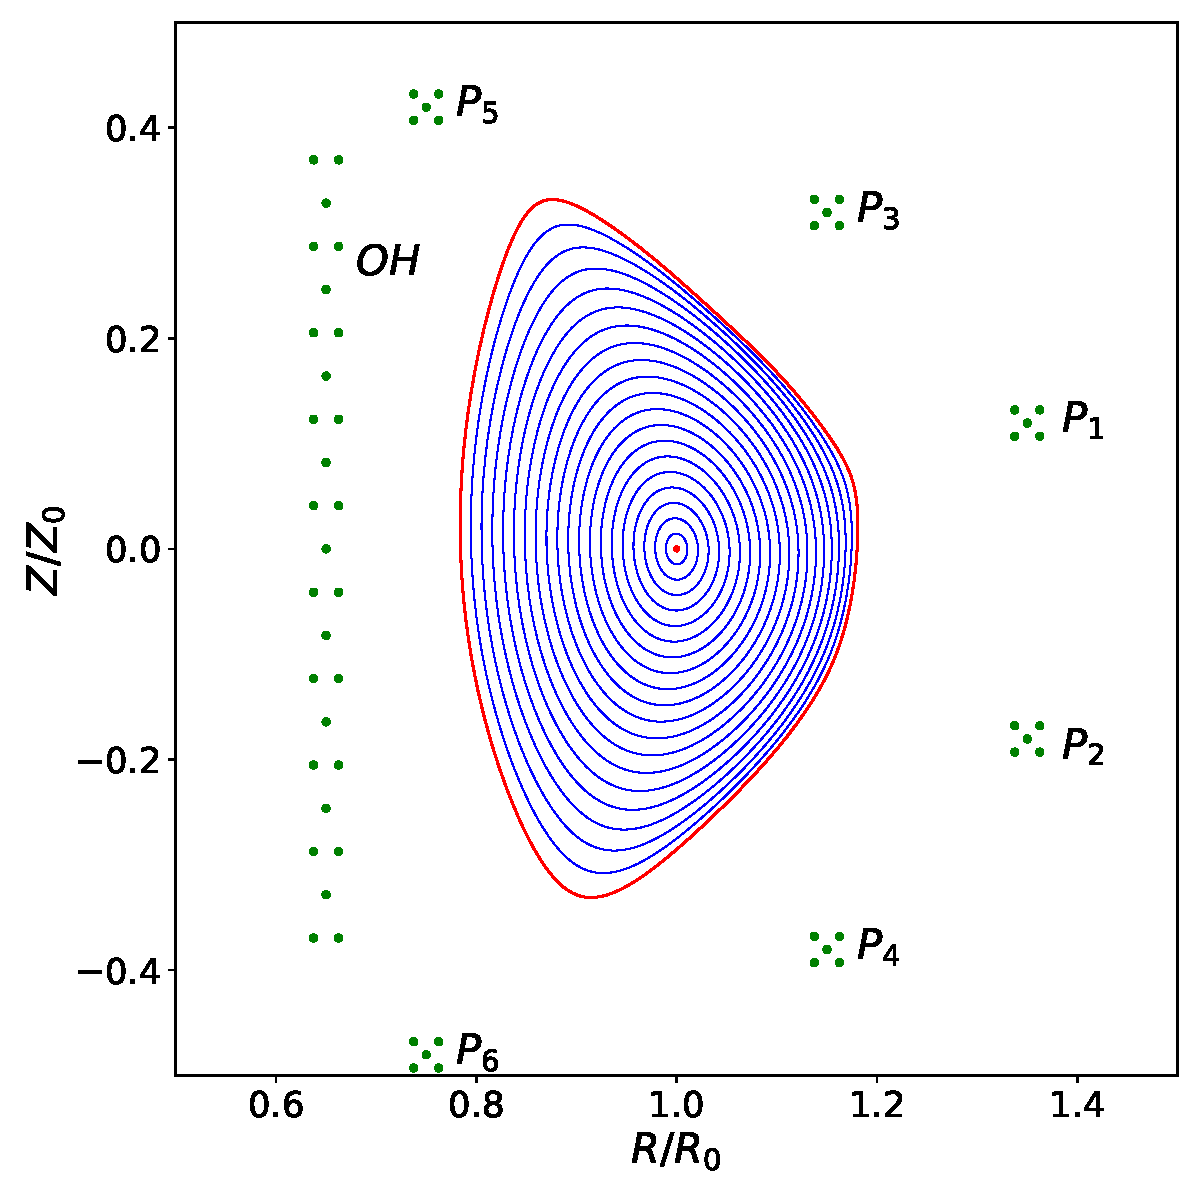
\includegraphics[width=0.8\textwidth]{Figure1.pdf}}
\caption{The blue curves show the internal magnetic flux-surfaces of an axisymmetric tokamak plasma equilibrium characterized by $\epsilon=0.25$, $q_c=1.0$, $\nu=3.0$, $p_c=0.25$, $\mu=2.1$, and ${\mit\Delta}_{\rm ped}=0$. 
The red curve denotes the plasma boundary, and the red dot corresponds to the magnetic axis. 
 Here, $OH$ is the ohmic heating coil, and $P_1$ through $P_6$ are the six poloidal field-coils.  Each green dot corresponds to a constituent strand (of zero poloidal cross-sectional area) of a given field-coil that carries the same toroidal current.
 The relative weights of the net toroidal currents flowing in $OH$ and $P_1$ to $P_6$ are $0.80$, $0.02$, $0.01$, $-0.01$, $-0.02$, $0.65$ and $0.75$, respectively.}\label{fig1}
\end{figure}

\begin{figure}
\centerline{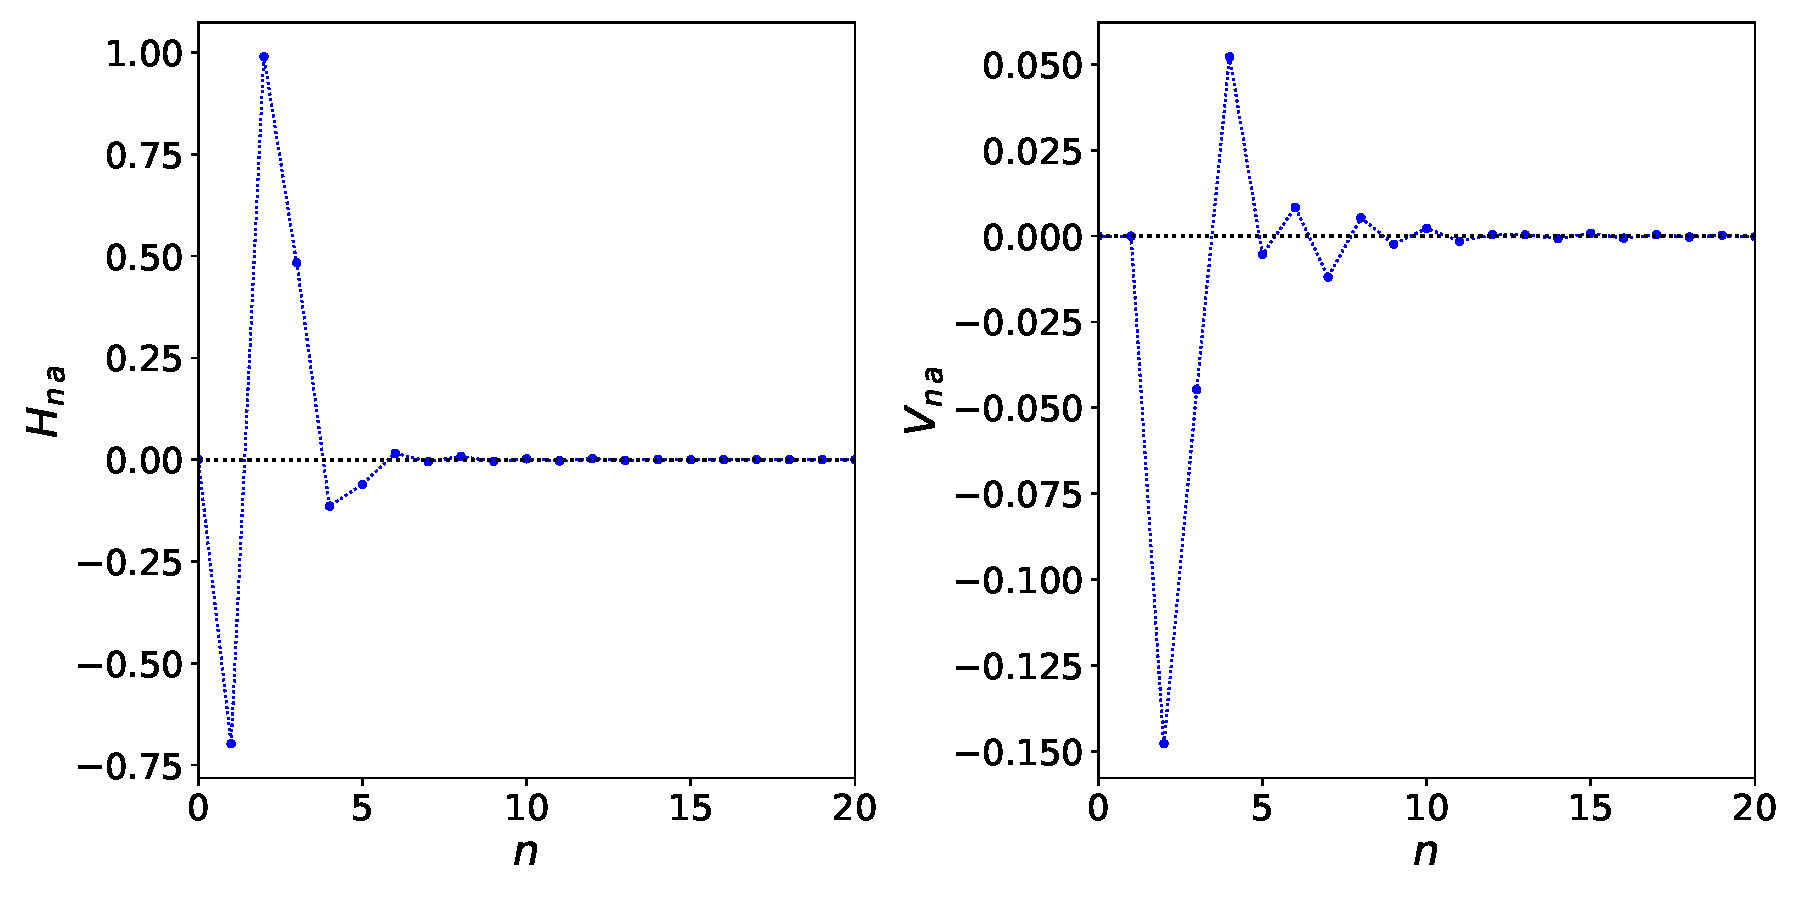
\includegraphics[width=\textwidth]{Figure2.pdf}}
\caption{Values of the shaping functions at the plasma boundary for the example tokamak plasma equilibrium shown in Fig.~\ref{fig1}.
Here, the $H_{n\,a}$ control the up-down symmetric shaping of magnetic flux-surfaces, whereas the $V_{n\,a}$ control the up-down
asymmetric shaping. Moreover, $n$ is a poloidal mode number.}\label{fig2}
\end{figure}

\begin{figure}
\centerline{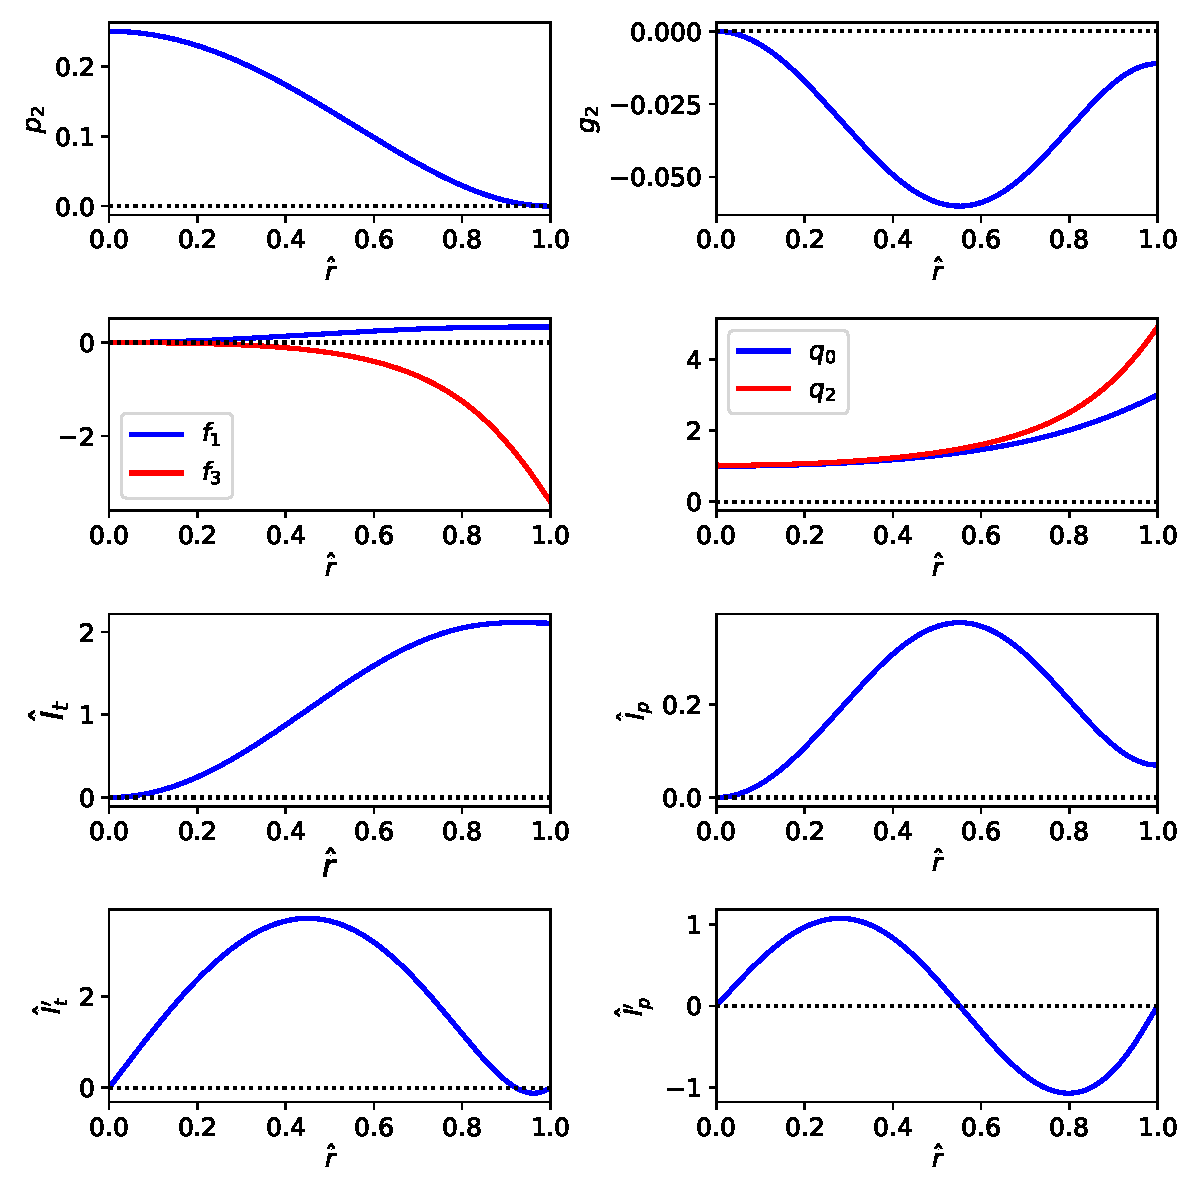
\includegraphics[width=\textwidth]{Figure3.pdf}}
\caption{Various characteristic profiles for the example tokamak plasma equilibrium shown in Fig.~\ref{fig1}.
Here, $p_2$ is the normalized plasma pressure profile, $g_2$ controls the variation of the toroidal magnetic
field-strength, $f_1$ and $f_3$ control the variation of the poloidal magnetic field-strength, $q_0$ and $q_2$ are the
lowest-order and corrected safety-factor profiles, respectively,  and $\hat{I}_t$ and $\hat{I}_p$ are the
normalized toroidal and poloidal currents, respectively, flowing within flux-surfaces. Finally, $\hat{r}$ is
a flux-surface label that is zero at the magnetic axis, and unity at the plasma boundary. }\label{fig3}
\end{figure}

\begin{figure}
\centerline{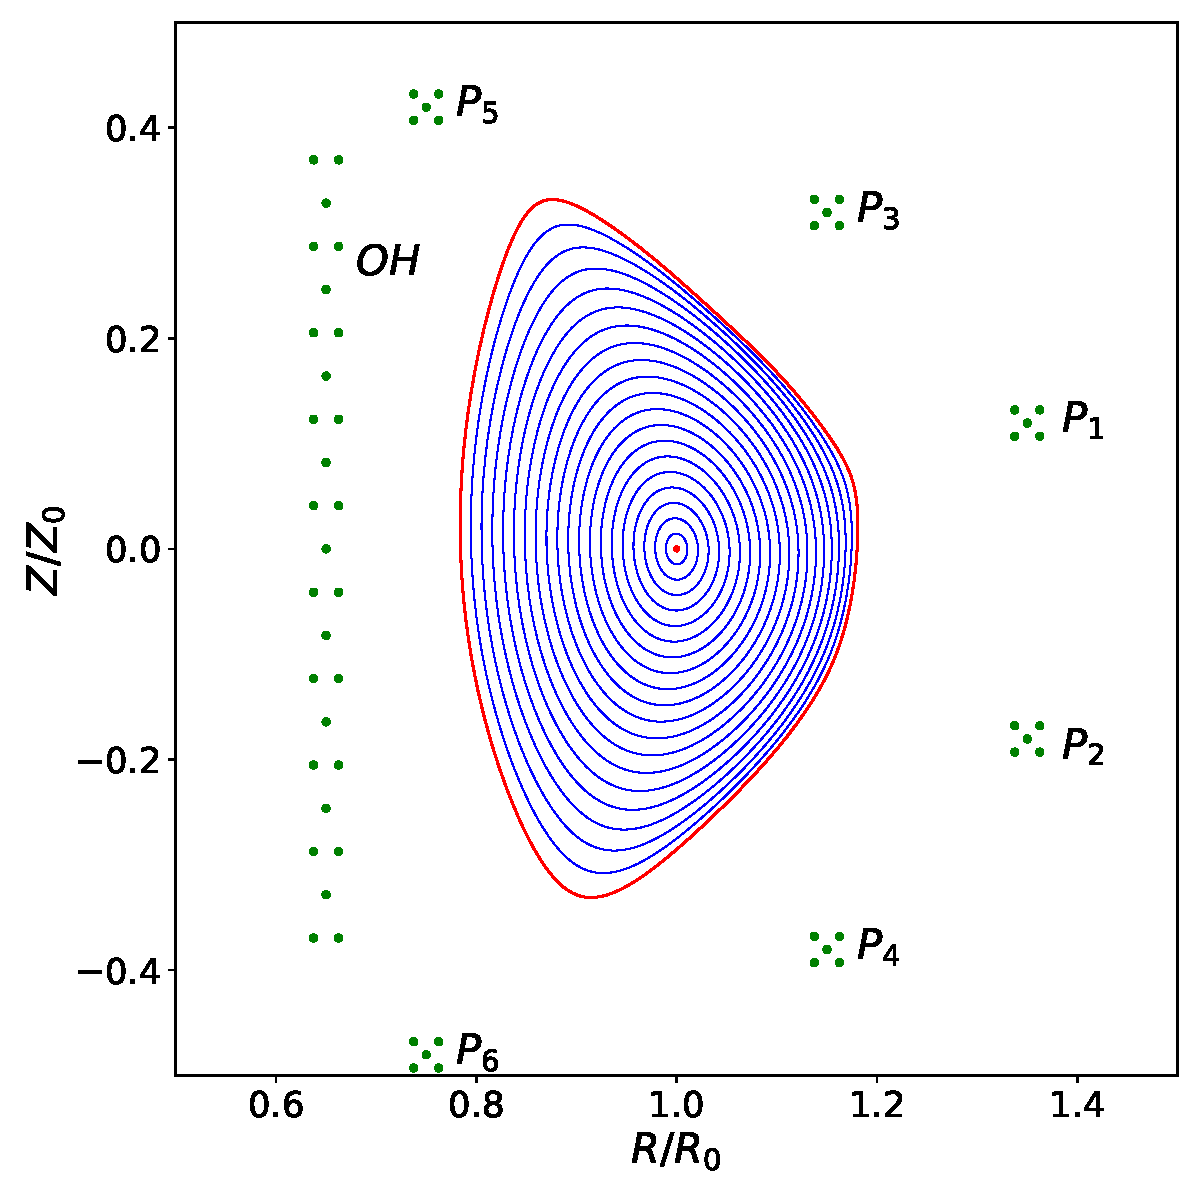
\includegraphics[width=0.8\textwidth]{Figure4.pdf}}
\caption{Internal magnetic flux-surfaces of a axisymmetric tokamak plasma equilibrium characterized by $\epsilon=0.25$, $q_c=1.0$, $\nu=3.0$, $p_c=0.25$, $\mu=2.1$,
${\mit\Delta}_{\rm ped}=0.05$, $\hat{\delta}_{\rm ped} = 0.025$, and $\hat{r}_{\rm ped}=0.95$.  See Fig.~\ref{fig1} caption. }\label{fig4}
\end{figure}

\begin{figure}
\centerline{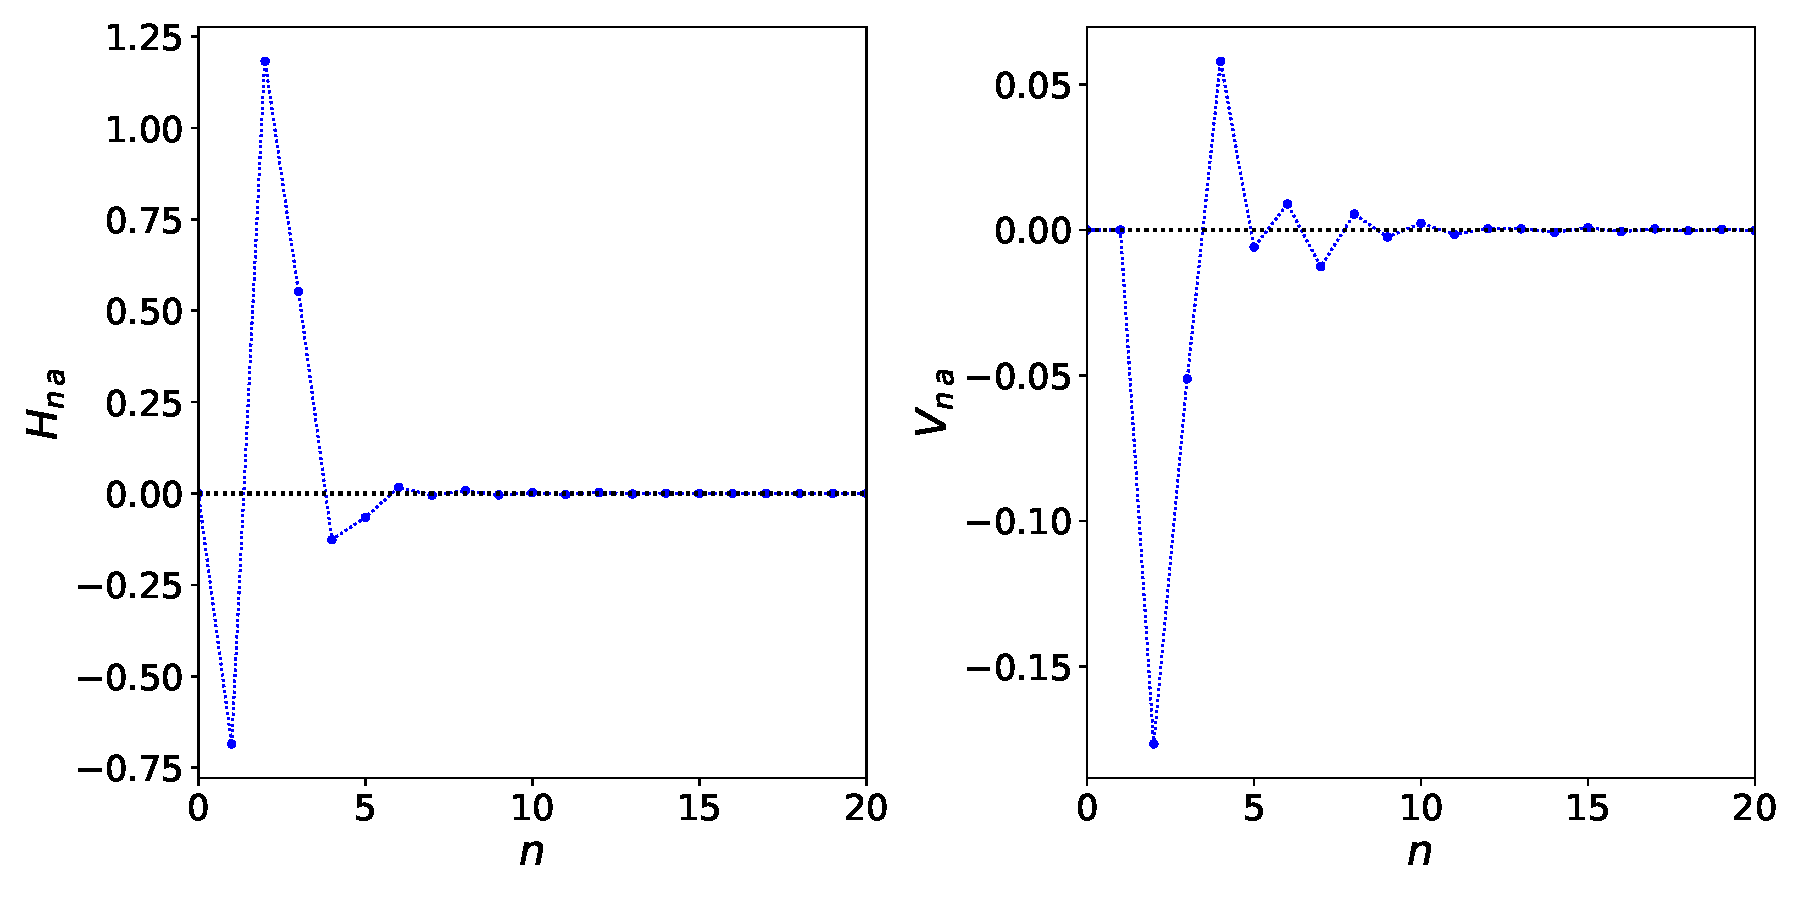
\includegraphics[width=\textwidth]{Figure5.pdf}}
\caption{Values of the shaping functions at the plasma boundary for the example tokamak equilibrium shown in Fig.~\ref{fig4}.
See Fig.~\ref{fig2} caption.}\label{fig5}
\end{figure}

\begin{figure}
\centerline{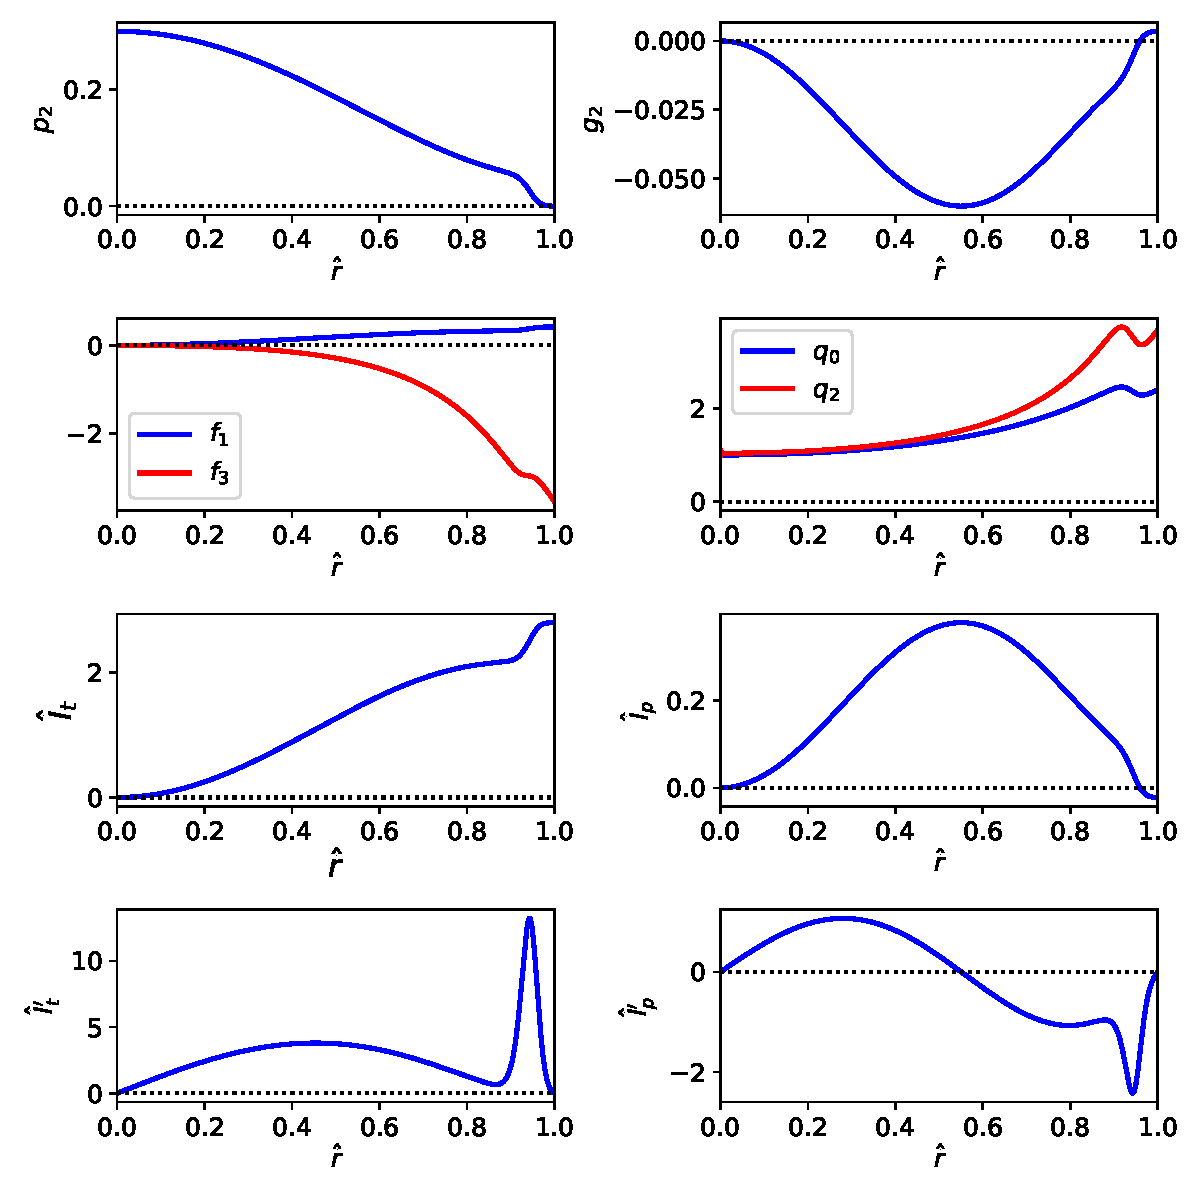
\includegraphics[width=\textwidth]{Figure6.pdf}}
\caption{Various characteristic profiles for the example tokamak equilibrium shown in Fig.~\ref{fig4}. See Fig.~\ref{fig3} caption.}\label{fig6}
\end{figure}

\end{document}


